\documentclass[11pt, spanish]{report}
\usepackage[spanish]{babel}
\selectlanguage{spanish}
\usepackage[utf8]{inputenc}
\usepackage{amssymb}
\usepackage{mathtools}
\usepackage{physics}
\usepackage{qcircuit}
\usepackage{graphicx}
\usepackage{float}
\usepackage{dsfont}
\usepackage{tkz-graph}
\usetikzlibrary{arrows}

\newcommand{\qwxo}[2][-1]{\ar @{-} [#1,0]|*+<4pt,6pt>[Fo]{#2}}


\begin{document}

\begin{abstract}
Your abstract goes here...
...
\end{abstract}
...

\chapter{Introducción}
La computación cuántica es como chévere

\chapter{Información cuántica}

\section{Kets, bras y operadores}

La notación bra-ket es la notación estándar en la mecánica cuántica para describir estados cuánticos. En el caso de la computación cuántica, se utilizan los kets $\ket{0}$ y $\ket{1}$ para describir los qubits en la base computacional. Este par de estados sería el equivalente a los bits 0 y 1 en la computación clásica. En su representación matricial, los kets $\ket{0}$ y $\ket{1}$ se representan de la siguiente manera:

\[\ket{0} = \begin{pmatrix} 1 \\ 0 \end{pmatrix}\]

\[\ket{1} = \begin{pmatrix} 0 \\ 1 \end{pmatrix}\]

Un bra es el operador adjunto de un ket. Los bras de la base computacional son $\bra{0}$ y $\bra{1}$. En la representación matricial estos son la transpuesta conjugada de los kets y se representan de la siguiente manera:

\[\bra{0} = \begin{pmatrix} 1 & 0 \end{pmatrix}\]

\[\bra{1} = \begin{pmatrix} 0 & 1 \end{pmatrix}\]

\section{Postulados de la mecánica cuántica}
\begin{enumerate}
\item Un estado puro en mecánica cuántica se representa en términos de
  un vector normalizado $\ket{\psi}$ en un espacio de Hilbert
  $\mathcal{H}$.
\item Si $\mathcal{H}_1$ y $\mathcal{H}_2$ son los espacios de Hilbert asociados a dos sistemas físicos, entonces el espacio del sistema
  compuesto $\mathcal{H}$ estará dado por el producto tensoral de los
  dos espacios de Hilbert
  $\mathcal{H} = \mathcal{H}_1 \otimes \mathcal{H}_2$.
\item Para todo observable $a$, existe un operador hermítico
  correspondiente $A$ que actua sobre el espacio de Hilbert
  $\mathcal{H}$, cuyos autovalores son los posibles resultados de una
  medida de este observable.
\item La evolución temporal del sistema sigue la ecuación de
  Schrödinger
  $i \hbar \frac{\partial \ket{\psi}}{\partial t} = H
  \ket{\psi}$. Donde $\hbar$ es la constante de Planck reducida y $H$
  es el Hamiltoniano del sistema, el cuál es el operador hermítico
  correspondiente a la energía.
\item Después de realizar una medida del observable $a$, el estado
  $\ket{\psi}$ del sistema colapsa a al autoestado de $A$
  correspondiente a la medida.
\end{enumerate}

\section{Computación cuántica}
This section's content...

\subsection{Qubits}
Un qubit es un sistema físico de dos niveles, es decir, es un objeto cuyo estado es un elemento del espacio de Hilbert de dimensión $\dim (\mathcal{H})=2$ y puede ser escrito de la siguiente manera: $ \ket{\psi} = \alpha \ket{0} + \beta \ket{1} $, donde $ \{ \ket{0},\ket{1} \} $ forma una base de $\mathcal{H}$ y donde $ \alpha $ y $ \beta $ son números complejos, tales que $ | \alpha |^2 + | \beta |^2 = 1 $, conocidos como amplitudes de probabilidad.

El qubit se puede pensar como el equivalente en IC del bit, el cual, por sus propiedad cuánticas, puede estar no sólo puede estar en el estado $\ket{0}$ y en el estado $\ket{1}$, sino también en superposiciones de estos dos.

El estado de un qubit también se puede escribir de la siguiente manera: $ \ket{\psi} = e^{i \phi_0} \cos ( \theta ) \ket{0} + e^{i \phi_1} \sin ( \theta ) \ket{1}  = e^{i \phi_0} (\cos ( \theta ) \ket{0} + e^{i ( \phi1 - \phi_0 )} \sin ( \theta ) \ket{1}) $, donde $ \theta $, $\phi_0$ y $\phi_1$ son números reales. La fase global $\phi_0$ es ignorable, pues no tiene ningún efecto sobre las probabilidades. Entonces, sin pérdida de generalidad, $ \ket{\psi} = \cos ( \theta ) \ket{0} + \sin ( \theta ) e^{i \phi} \ket{1} $, donde $ \theta \in [0, \pi ] $ y $ \phi \in [0, 2 \pi ] $. De esta manera, podemos representar los qubits en una esfera unitaria, conocida como esfera de Bloch.

\subsection{Compuertas cuánticas}
Las operaciones unitarias con las que se opera sobre los qubits reciben el nombre de compuertas cuánticas.

Las compuertas de un sólo qubit pueden ser vistas como rotaciones en la esfera de Bloch.

\subsubsection{Compuerta identidad}

Esta operación es equivalente a \textit{no-operation} en una computadora clásica.

\begin{minipage}{0.5\textwidth}
\[
\Qcircuit @C=1.4em @R=1.8em {
& \gate{I} & \qw
}
\]
\end{minipage}
\begin{minipage}{0.5\textwidth}
\[
\begin{pmatrix}
1 & 0 \\
0 & 1
\end{pmatrix}
\]
\end{minipage}

\subsubsection{Compuerta X}
Este es el equivalente al NOT clásico, pues tránsforma los $\ket{0}$ en $\ket{1}$ y viceversa, ya que realiza una rotación de $\pi$ sobre el eje X en la esfera de Bloch. Su forma matricial viene dada por la matriz de Pauli $\sigma_x$

\begin{minipage}{0.5\textwidth}
\[
\Qcircuit @C=1.4em @R=1.8em {
& \gate{X} & \qw
}
\]
\end{minipage}
\begin{minipage}{0.5\textwidth}
\[
\begin{pmatrix}
0 & 1 \\
1 & 0
\end{pmatrix}
\]
\end{minipage}

\subsubsection{Compuerta Z}
Esta compuerta no tiene análogo clásico, pues lo que realiza es un cambio de fase. Esto equivale a una rotación de $\pi$ sobre el eje Z en la esfera de Bloch. Su forma matricial viene dada por la matriz de Pauli $\sigma_z$

\begin{minipage}{0.5\textwidth}
\[
\Qcircuit @C=1.4em @R=1.8em {
& \gate{Z} & \qw
}
\]
\end{minipage}
\begin{minipage}{0.5\textwidth}
\[
\begin{pmatrix}
1 & 0 \\
0 & -1
\end{pmatrix}
\]
\end{minipage}

\subsubsection{Compuerta Y}
Esta compuerta realiza una rotación de $\pi$ sobre el eje y de la esfera de Bloch. Su forma matricial viene dada por la matriz de Pauli $\sigma_y$

\begin{minipage}{0.5\textwidth}
\[
\Qcircuit @C=1.4em @R=1.8em {
& \gate{Y} & \qw
}
\]
\end{minipage}
\begin{minipage}{0.5\textwidth}
\[
\begin{pmatrix}
0 & -i \\
i & 0
\end{pmatrix}
\]
\end{minipage}

\subsubsection{Compuerta de Hadamard}
%Esta compuerta realiza una rotación de $\frac{\pi}{2}$ sobre el eje y de la esfera de Bloch. Ella es de especial importancia, pues transforma los estados de la base computacional $\ket{0}$ y $\ket{1}$ en estados de superposiciones uniformes ($\ket{+}$ y $\ket{-}$). También se puede interpretar como el mapa de la base Z a la base X.
Esta compuerta transforma los estados de la base computacional $\ket{0}$ y $\ket{1}$ en estados de superposiciones uniformes ($\ket{+}$ y $\ket{-}$). También se puede interpretar como el mapa de la base Z a la base X.

\begin{minipage}{0.5\textwidth}
\[
\Qcircuit @C=1.4em @R=1.8em {
& \gate{H} & \qw
}
\]
\end{minipage}
\begin{minipage}{0.5\textwidth}
\[
\frac{1}{\sqrt{2}}
\begin{pmatrix}
1 & 1 \\
1 & -1
\end{pmatrix}
\]
\end{minipage}

\subsubsection{Compuerta S}
Esta compuerta es la raiz cuadrada de Z.

\begin{minipage}{0.5\textwidth}
\[
\Qcircuit @C=1.4em @R=1.8em {
& \gate{S} & \qw
}
\]
\end{minipage}
\begin{minipage}{0.5\textwidth}
\[
\begin{pmatrix}
1 & 0 \\
0 & i
\end{pmatrix}
\]
\end{minipage}

\subsubsection{Compuerta T}
Esta compuerta es la raiz cuadrada de S.

\begin{minipage}{0.5\textwidth}
\[
\Qcircuit @C=1.4em @R=1.8em {
& \gate{T} & \qw
}
\]
\end{minipage}
\begin{minipage}{0.5\textwidth}
\[
\begin{pmatrix}
1 & 0 \\
0 & e^{\frac{i \pi}{4}}
\end{pmatrix}
\]
\end{minipage}

\subsubsection{Compuerta de cambio de fase}

\begin{minipage}{0.5\textwidth}
\[
\Qcircuit @C=1.4em @R=1.8em {
& \gate{R_{\phi}} & \qw
}
\]
\end{minipage}
\begin{minipage}{0.5\textwidth}
\[
\begin{pmatrix}
1 & 0 \\
0 & e^{i \phi}
\end{pmatrix}
\]
\end{minipage}

\subsubsection{Compuertas de rotación}

\[
R(\theta,\vec{r}) = e^{i \frac{\theta}{2} \vec{\sigma} \cdot \vec{r}} =
\begin{pmatrix}
\cos(\frac{\theta}{2}) + i z \sin(\frac{\theta}{2}) & \sin(\frac{\theta}{2}) (i x + y) \\
\sin(\frac{\theta}{2}) (i x - y) & \cos(\frac{\theta}{2}) - i z \sin(\frac{\theta}{2})
\end{pmatrix}
\]

\[
R_y(\theta) =
\begin{pmatrix}
\cos(\frac{\theta}{2}) & \sin(\frac{\theta}{2}) \\
-\sin(\frac{\theta}{2}) & \cos(\frac{\theta}{2})
\end{pmatrix}
\]

\[
R_z(\theta) =
\begin{pmatrix}
e^{i \frac{\theta}{2}} & 0 \\
0 & e^{-i \frac{\theta}{2}}
\end{pmatrix}
\]

\[
R_x(\theta) =
\begin{pmatrix}
\cos(\frac{\theta}{2}) & i \sin(\frac{\theta}{2}) \\
i\sin(\frac{\theta}{2}) & \cos(\frac{\theta}{2})
\end{pmatrix}
\]

\[
R_x(\theta) = R_z(\frac{\pi}{2}) R_y(\theta) R_z(\frac{-\pi}{2})
\]

\subsubsection{Compuerta CNOT}

\begin{minipage}{0.5\textwidth}
\[
\Qcircuit @C=1.4em @R=1.8em {
& \ctrl{1} & \qw \\
& \targ & \qw \\
}
\]
\end{minipage}
\begin{minipage}{0.5\textwidth}
\[
\begin{pmatrix}
1 & 0 & 0 & 0 \\
0 & 1 & 0 & 0 \\
0 & 0 & 0 & 1 \\
0 & 0 & 1 & 0
\end{pmatrix}
\]
\end{minipage}

\subsubsection{Compuerta SWAP}

\begin{minipage}{0.5\textwidth}
\[
\Qcircuit @C=1.4em @R=1.8em {
& \qswap & \qw \\
& \qswap \qwx & \qw \\
}
\]
\end{minipage}
\begin{minipage}{0.5\textwidth}
\[
\begin{pmatrix}
1 & 0 & 0 & 0 \\
0 & 0 & 1 & 0 \\
0 & 1 & 0 & 0 \\
0 & 0 & 0 & 1
\end{pmatrix}
\]
\end{minipage}

\subsubsection{Compuerta $\sqrt{\text{SWAP}}$}

\begin{minipage}{0.5\textwidth}
\[
\Qcircuit @C=1.4em @R=1.8em {
& \qswap & \qw \\
& \qswap\qwxo{\scalebox{0.5}{$1\hspace{-1pt}/\hspace{-1pt}2$}} & \qw
}
\]
\end{minipage}
\begin{minipage}{0.5\textwidth}
\[
\begin{pmatrix}
1 & 0 & 0 & 0 \\
0 & \frac{1}{2} (1+i) & \frac{1}{2} (1-i) & 0 \\
0 & \frac{1}{2} (1-i) & \frac{1}{2} (1+i) & 0 \\
0 & 0 & 0 & 1
\end{pmatrix}
\]
\end{minipage}

\subsubsection{Compuerta de Ising}

\begin{minipage}{0.5\textwidth}
\[
\Qcircuit @C=1.4em @R=1.8em {
& \multigate{1}{\mathit{XX}_{\phi}} & \qw \\
& \ghost{\mathit{XX}_{\phi}} & \qw
}
\]
\end{minipage}
\begin{minipage}{0.5\textwidth}
\[
\frac{1}{\sqrt{2}}
\begin{pmatrix}
1 & 0 & 0 & -i e^{i \phi} \\
0 & 1 & -i & 0 \\
0 & -i & 1 & 0 \\
-i e^{-i \phi} & 0 & 0 & 1
\end{pmatrix}
\]
\end{minipage}

\subsubsection{Compuerta de Toffoli}

\begin{minipage}{0.5\textwidth}
\[
\Qcircuit @C=1.4em @R=1.8em {
& \ctrl{1} & \qw \\
& \ctrl{1} & \qw \\
& \targ & \qw \\
}
\]
\end{minipage}
\begin{minipage}{0.5\textwidth}
\[
\begin{pmatrix}
1 & 0 & 0 & 0 & 0 & 0 & 0 & 0 \\
0 & 1 & 0 & 0 & 0 & 0 & 0 & 0 \\
0 & 0 & 1 & 0 & 0 & 0 & 0 & 0 \\
0 & 0 & 0 & 1 & 0 & 0 & 0 & 0 \\
0 & 0 & 0 & 0 & 1 & 0 & 0 & 0 \\
0 & 0 & 0 & 0 & 0 & 1 & 0 & 0 \\
0 & 0 & 0 & 0 & 0 & 0 & 0 & 1 \\
0 & 0 & 0 & 0 & 0 & 0 & 1 & 0
\end{pmatrix}
\]
\end{minipage}

\subsubsection{Compuerta de Fredkin}

\subsubsection{Compuerta de Deutsch}

\begin{minipage}{0.5\textwidth}
\[
\Qcircuit @C=1.4em @R=1.8em {
& \multigate{2}{D(\theta)} & \qw \\
& \ghost{D(\theta)} & \qw \\
& \ghost{D(\theta)} & \qw
}
\]
\end{minipage}
\begin{minipage}{0.5\textwidth}
\[
\begin{pmatrix}
1 & 0 & 0 & 0 & 0 & 0 & 0 & 0 \\
0 & 1 & 0 & 0 & 0 & 0 & 0 & 0 \\
0 & 0 & 1 & 0 & 0 & 0 & 0 & 0 \\
0 & 0 & 0 & 1 & 0 & 0 & 0 & 0 \\
0 & 0 & 0 & 0 & 1 & 0 & 0 & 0 \\
0 & 0 & 0 & 0 & 0 & 1 & 0 & 0 \\
0 & 0 & 0 & 0 & 0 & 0 & i \cos(\theta) & \sin(\theta) \\
0 & 0 & 0 & 0 & 0 & 0 & \sin(\theta) & i \cos(\theta)
\end{pmatrix}
\]
\end{minipage}

\[
\ket{a,b,c} \rightarrow
\begin{cases}
i \cos(\theta) \ket{a,b,c} + \sin(\theta) \ket{a,b,c \oplus 1} & \text{si } a=b=1 \\
\ket{a,b,c} & \text{en otro caso}
\end{cases}
\]

\subsection{Correspondencia entre compuertas clásicas y cuánticas}

\subsection{Conjuntos universales de compuertas cuánticas}
Un conjunto universal de compuertas cuánticas (CUCC) es un conjunto finito de compuertas cuánticas con el cuál se puede aproximar cualquier operación unitaria arbitrariamente bien.

Cualquier operador unitario puede ser escrito en función de compuertas de uno y dos qubits [Barenco et al. 1995].

Un CUCC simple es $\{H,T,\mathit{CNOT}\}$.

Existe un CUCC de una sóla compuerta, la compuerta de Deutsch, $D(\theta)$.

La compuerta de Toffoli es un caso especial de la compuerta de Deutsch, $D(\frac{\pi}{2})$.

Otro CUCC consiste en la compuerta de Ising y la compuerta de cambio de fase, \{$\mathit{XX}_\phi,R_z(\theta)$\}. Este conjunto es nativo en algunas computadoras cuánticas de trampas de iones.

\subsection{Compuertas no cliffordianas}
Las compuertas cliffor


\subsection{Circuitos cuánticos}

\subsection{Paralelismo cuántico}

\subsection{Algoritmos cuánticos}

\subsection{Criterios de DiVincenzo}
Para construir un computador cuántico, se deben cumplir las siguientes condiciones experimentales:

\begin{enumerate}
\item Un sistema físico escalable con qubits bien caracterizados.
\item La habilidad de inicializar el estado de los qubits en un estado fiducial simple.
\item Tiempos de coherencia relevantes largos.
\item Un conjunto universal de compuertas cuánticas.
\item La capacidad de medir qubits en específico.
\end{enumerate}

\chapter{Superconductividad}
Los qubits superconductores se basan en circuitos osciladores no lineales, hechos a partir de uniones de Josephson (Josephson Junctions - JJ). [Wendin]

El Hamiltoniano de un oscilador armónico LC está dado por 

\[
\hat{H} = E_C \hat{n}^2 + E_L \frac{\hat{\phi}^2}{2},
\]

donde $\hat{n}$ es la cantidad de pares de Cooper inducidos en el capacitor (En otras parabras, la carga inducida en el capacitor, medida en unidades de $2e$), y $\hat{\phi}$ es la diferencia de fase sobre el inductor. La carga $\hat{n}$ y la fase $\hat{\phi}$ no conmutan, $\comm{\hat{\phi}}{\hat{n}}=i$, lo que significa que sus valores esperados no se pueden medir simultaneamente. $E_C=\frac{(2e)^2}{2C}$, $E_L=\frac{\hbar^2}{(2e)^2L}$ y la distancia entre niveles de energía del oscilador armónico $\hbar \omega = \frac{\hbar}{\sqrt{LC}}=\sqrt{2E_LE_C}$.

Para poder servir como qubit, el oscilador debe ser anarmónico, de manera que se pueda operar sobre un par específico de niveles de energía. Al agregar una JJ, el Hamiltoniano del circuito LCJ se convierte en:

\[
\hat{H} = E_C (\hat{n}-n_g)^2 - E_{J0} \cos( \hat{\phi} ) + E_L \frac{(\hat{\phi}-\phi_e)^2}{2},
\]

donde $n_g$ es la carga inducida por voltaje en el capacitor C (isla qubit) y $\phi_e$ es la fase inducida por flujo sobre la JJ. La energía de Josephson $E_{J0}$ está dada por $E_{J0}=\frac{\hbar}{2e}I_0$ en términos de la corriente crítica $I_0$ de la unión. Usualmente, la JJ es del tipo Superconductor-Aislante-Superconductor con corriente crítica fija.

Con el fin de introducir la inductancia no lineal de Josephson, empezamos por 

\[
I_J = I_0 \sin(\phi)
\]

Combinado con la ley de Lenz:

\[
V = \frac{d\Phi}{dt} = \frac{\Phi_0}{2\pi} \frac{d\phi}{dt}, \hspace{20pt} \Phi_0=\frac{h}{2e}
\]

Se encuentra que:

\[
V = \frac{\Phi_0}{2\pi} \frac{1}{I_0\cos(\phi)} \frac{dI_J}{dt}
\]

Definiendo $L_J = V (\frac{dI_J}{dt})^{-1}$, se obtiene finalmente la inductancia de Josephson $L_{J0}$:

\[
L_J = \frac{\Phi_0}{2\pi} \frac{1}{I_0 \cos(\phi)} = L_{J0} \frac{1}{\cos(\phi)}
\]

Esto define la inductancia de Josephson de la JJ aislada y nos permite expresar la energía de Josephson como $E_{J0} = \frac{\hbar^2}{(2e)^2L_{J0}}$

\begin{align*}
[E_C (-i\hbar \frac{\partial}{\partial\phi}-n_g)^2 + U(\phi)] \psi = E \psi \\
U(\phi) = -E_{J0} \cos(\phi) + E_L \frac{(\phi-\phi_e)^2}{2}
\end{align*}

\begin{enumerate}
\item $E_L = 0 \quad (L \sim \infty)$ :
\item $E_L \approx E_{J0}$ :
\end{enumerate}

\section{Transmonios}
Tratando el transmonio como un sistema de dos niveles acoplado linealmente a un oscilador monomodo, su Hamiltoniano toma la siguiente forma:

\[
\hat{H} = \hat{H}_q + \hat{H}_{qr} + \hat{H}_r = -\frac{1}{2} \epsilon \sigma_z + g \sigma_x (a+a^\dag) + \hbar \omega (a^\dag a + \frac{1}{2})
\]

donde $\epsilon$ es la energía de excitación del qubit, $g$ es el acoplamiento qubit-oscilador y $\omega$ es la frecuencia del oscilador.

Introduciendo los operadores escalera del qubit, $\sigma_\pm = \frac{1}{2}(\sigma_x \pm i \sigma_y)$, el término de interacción $\hat{H}_{qr}$ se puede dividir en dos términos, el de Jaynes-Cummings (JC) y el anti-Jaynes-Cummings (AJC):

\[
\hat{H}_{qr} = \hat{H}_{qr}^{JC} + \hat{H}_{qr}^{AJC} = g(\sigma_+ a + \sigma_- a^\dag) + g(\sigma_+ a^\dag + \sigma_- a)
\]

Este Hamiltoniano describe el modelo cuántico canónico de Rabi (canonical quantum Rabi model - QRM). Las ecuaciones ()() son completamente generales y aplicables a cualquier sistema qubit-oscilador. Mantener sólo el término JC correponde a realizar la aproximación de onda rotativa (rotating wave approximation - RWA).

\section{Hamiltonianos multiqubit de transmonios}
Omitiendo el término del oscilador, el Hamiltoniano toma la siguiente forma general:

\[
\hat{H} = \hat{H}_q + \hat{H}_{qr} + \hat{H}_{qq} = -\frac{1}{2} \sum\limits_i \epsilon_i \sigma_{zi} + \sum\limits_i g_i \sigma_{xi} (a+a^\dag) + \frac{1}{2} \sum\limits_{i,j;\nu} \lambda_{\nu,ij} \sigma_{\nu i} \sigma_{\nu j}
\]

Por simplicidad, se considera que el término $\hat{H}_{qr}$ se refiere sólo a la lectura y las operaciones de bus, dejando la interacción indirecta qubit-qubit via el resonador ser incluidas en $\hat{H}_{qq}$ via la constante de acoplamiento $\lambda_{\nu,ij}$.

\subsection{Acoplamiento capacitivo}
\begin{align*}
\hat{H}_{qq} = \lambda_{1 2} \sigma_{x1} \sigma_{x2} \\
\lambda_{1 2} = \frac{1}{2} \sqrt{E_{1 0, 1} E_{1 0, 2}} \frac{\sqrt{E_{E_{C1}} E_{E_{C2}}}}{E_{Cc}} = \frac{1}{2} \sqrt{E_{1 0, 1} E_{1 0, 2}} \frac{Cc}{\sqrt{C_1 C_2}} \approx \frac{1}{2} E_{1 0} \frac{C_c}{C} \\
\hat{H}_{qq} = \lambda_{1 2} (\sigma_{+1} \sigma_{-2}  + \sigma_{-1} \sigma_{+2})
\end{align*}

\subsection{Acoplamiento por el resonador}
\begin{align*}
\hat{H}_{qq} = \lambda_{1 2} \sigma_{x1} \sigma_{x2} \\
\lambda{1 2} = \frac{1}{2} g_1 g_2 (\frac{1}{\Delta_1} + \frac{1}{\Delta_2} \equiv g_1 g_2 \frac{1}{\Delta}) \\
\Delta_i = \epsilon_i - \hbar \omega
\end{align*}

\subsection{Acoplamiento de JJ}
\begin{align*}
\hat{H}_{qq} = \lambda_{1 2} \sigma_{y1} \sigma_{y2} \\
\lambda_{1 2} \approx \frac{1}{2} E_{1 0} \frac{L_c}{L_J} \frac{\cos(\delta_c)}{2L_c \cos(\delta_c) + L_{J c}}
\end{align*}

\subsection{Acoplamiento afinable/calibrable}

\section{Compuertas cuánticas en transmonios}

\subsection{El operador de evolución temporal}
La evolución temporal de un sistema complejo (many-body) puede ser descrita por la ecuación de Schrödinger para el vector de estado $\ket{\psi(t)}$:

\[
i \hbar \frac{\partial}{\partial t} \ket{\psi(t)} = \hat{H}(t) \ket{\phi(t)}
\]

en términos del operador evolución $\hat{U}(t,t_0)$

\[
\ket{\psi(t)} = \hat{U}(t,t_0) \ket{\psi(t_0)}
\]

determinado a partir del Hamiltoniano complejo (many-body) dependiente del tiempo del sistema:

\[
\hat{H} = \hat{H}_{syst} + \hat{H}_{ctrl}(t)
\]

describiendo el sistema intrínseco y las operaciones de control aplicadas. Las compuertas son el resultado de aplicar pulsos de control específicos a partes selectas de un circuito físico. Esto afecta varios términos del Hamiltoniano, haciéndolos dependientes del tiempo.

Para el transmonio, el Hamiltoniano del sistema bajo la RWA toma la forma:

\[
\hat{H}_{syst} = -\frac{1}{2} \sum\limits_{\nu i} \epsilon_i \sigma_{z i} + \sum\limits_{i} g_i (\sigma_{+ i} a + \sigma_{- i} a^\dag) + \hbar \omega a^\dag a + \frac{1}{2} \sum\limits_{i,j;\nu} \lambda_{\nu, ij} (\sigma_{+ i} \sigma_{- j} + \sigma_{- i} \sigma_{+ j})
\]

y el término de control se puede escribir como:

\[
\hat{H}_{ctrl} = \sum\limits_{i; \nu} f_{\nu i}(t) \sigma_{\nu i} + \frac{1}{2} \sum\limits_{i,j;\nu} h_{\nu, ij}(t) \sigma_{\nu i} \sigma_{\nu j} + k(t) a^\dag a
\]



\chapter{Algoritmo de Grover}
%El algoritmo de Grover es un AC que encuentra con alta probabilidad la entrada única de una función de caja negra que produce un valor particular de salida, usando tan sólo $O(\sqrt{N})$ evaluaciones de la función, donde $N$ es el tamaño del dominio de la función. El análogo clásico de este algoritmo requiere $O(N)$ evaluaciones de la función, pues, el elemento correcto podría ser el $N$-ésimo en ser evaluado y se deben evaluar uno por uno. La aplicación directa de este algoritmo es como algoritmo de búsqueda en una base de datos. Sin embargo, su aplicación más eficiente es como subrutina en diversos procesos de optimización.

El algoritmo de Grover es un AC que realiza una búsqueda en una secuencia no ordenada de datos con $N=2^n$ entradas. Clásicamente esta búsqueda tendría un orden de complejidad de $O(N)$, pues, como los datos no están ordenados, la cantidad promedio de evaluaciones que se deben realizar crece linealmente con la cantidad de entradas. En el caso del algoritmo de Grover, la complejidad de la búsqueda es de $O(\sqrt{N})$, pues se requieren aproximadamente $\frac{\pi\sqrt{N}}{4}$ iteraciones para hallar la entrada deseada. En cuanto a la cantidad de qubits requeridos, se necesitan $O(\log_2 N)$ qubits, pues se debe realizar un estado superpuesto donde cada componente de la superposición represente una entrada de la secuencia de datos.

Introducción:

Dada $f:{0,1}^n \rightarrow {0,1}$, es decir; $f:{0,1,2,...,N-1} \rightarrow
{0,1}$, se tiene la promesa de que 
\[
  f(x) = 
\begin{cases}
1 & \text{si } x = x_0 \\
0 & \text{si } x \neq x_0
\end{cases}
\]

Hay que determinar $x$.

Clásicamente hay que evaluar la función $N=2^n$ veces. Cuánticamente sólo se
requiere evaluar $\sqrt{2^n}$ veces.

El análisis usual del algoritmo de Grover se basa en un hecho bien conocido de
la geometría plana elemental: ``El producto de dos reflexiones es una rotación''

Veamos qué significa esto:

Supongamos que tenemos el oráculo

\[U_f \ket{x} = (-1)^{f(x)} \ket{x} =
    \begin{cases}
      \ket{x} & \text{si } x \neq x_0 \\
      - \ket{x} & \text{si } x = x_0
    \end{cases}\]

Es decir: $U_f = \mathds{1} - 2 \ketbra{x_0}{x_0}$
  
El efecto de $U_f$ es invertir la componente de $\ket{\phi}$ en la dirección
$\ket{x_0}$.

Además, podemos definir otro operador unitario $U_s = -\mathds{1} + 2
\ketbra{s}{s}$ donde $\ket{s} = H^{\otimes n} \ket{0} = \frac{1}{\sqrt{2^n}}
\sum\limits_x \ket{x}$

El efecto de $U_s$ es invertir todas las componentes en direcciones
perpendiculares a $\ket{s}$. Es decir, refleja respecto de $\ket{s}$.

Hagamos ahora el siguiente ejercicio:

Cosidremos el estado inicial $\ket{\psi}$

\begin{enumerate}
\item Aplicamos $U_\omega$, que invierte la componente $\ket{x_0}$.
\item Aplicamos $U_s$, que refleja respecto de $\ket{s}$
\end{enumerate}

La combinación de estas dos inversiones es una rotación en un ángulo $2\alpha$.

%%%%%% INSERTAR GRÁFICAS DEL EJEMPLO %%%%%%

Una vez entendido esto empecemos el algoritmo de Grover.

Algoritmo de Grover:

Asumamos que el tamaño de nuestra base de datos es $2^n \equiv N$, donde $n$ es cualquier número entero distinto de creo.

Consideremos un observable $\Omega \in H$ de dimensión $N \geq 2$. Este
observable define un conjunto de bases ortogonales $\ket{x} = \{\ket{0},
\ket{1}, \ket{2},...,\ket{N-1}\}$ con autovalores conocidos $\lambda_0,
\lambda_1, \lambda_2,..., \lambda_{N-1}$, tal que $\hat{\Omega} \ket{j} =
\lambda_j \ket{j}$, $j \in {0,...,N-1}$.

Entonces podemos asociar un único autoestado $\ket{x_j}$, o autovalor
$\lambda_j$, con cada item en la base de datos.

El problema de buscar en la base de datos se convierte ahora en el problema de
medir un autovalor de interés al que llamaremos $\lambda_\omega$, asociado con
el estado $\ket{\omega}$, el cual representa algún específico item $\omega$ en
nuestra base de datos y el cuál deseamos encontrar usando el algoritmo de
búsqueda de Grover.

Entonces:

$$\{\ket{x}\}_{x=0,1,...,N-1} \text{es ortonormal }\rightarrow \ket{s} =
\frac{1}{\sqrt{N}} \sum\limits_{x=0}^{N-1} \ket{x} = \text{autoestado asociado a
  la base de datos}$$

$$\braket{s}{s} = 1 \text{ ya que } \braket{i}{j} = \delta_{ij}$$

Cualquier autoestado $\ket{\omega}$ tiene la misma proyección
$\braket{\omega}{s} = \frac{1}{sqrt{N}}$, y dado un item $\omega$ la
probabilidad de medir $\lambda_\omega$ (que es equivaletne a encontrar $\ket{s}$
en el estado $\ket{\omega}$) es $|\braket{\omega}{s}|^2 = \frac{1}{N}$,
consistentemente con lo que ocurre con una base de datos clásica.

Consideremos ahora el oráculo unitario $U_\omega$ definido como:

$$U_\omega \equiv \mathds{1} - 2\ketbra{\omega}{\omega}$$

Entonces $U_\omega \ket{x} = (\mathds{1} - 2\ketbra{\omega}{\omega}) \ket{x} =
\ket{x} - 2 \braket{\omega}{x} \ket{\omega} = \ket{x} - 2 \delta_{ij} \ket{\omega}$
 Si $x \neq \omega \rightarrow U_\omega \ket{x} = \ket{x}$ 
 Si $x = \omega \rightarrow U_\omega \ket{x} = -\ket{\omega}$ 

De manera tal que $U_\omega \ket{s} = U_\omega (\frac{1}{\sqrt{N}}
\sum\limits_{x = 0}^{N-1}) = \frac{1}{\sqrt{N})} U_\omega (\sum\limits_{x=0,
  x\neq\omega}^{N-1} \ket{x} + \ket{\omega}) =
\frac{1}{\sqrt{N}}\sum\limits_{x=0, x\neq\omega}^{N-1} \ket{x} -
\frac{1}{\sqrt{N}} \ket{\omega}$.

Esto se puede reescribir como:

$U_\omega \ket{s} = \frac{1}{\sqrt{N}} \sum\limits_{x=0, x\neq\omega}^{N-1}
\ket{x} + (\frac{1}{\sqrt{N}} \ket{\omega} - \frac{1}{\sqrt{N}} \ket{\omega} )- \frac{1}{\sqrt{N}} \ket{\omega} $

Por lo tanto: $U_\omega \ket{s} = \frac{1}{\sqrt{N}} \sum_{x=0}^{N-1} \ket{x} -
\frac{2}{\sqrt{N}} \ket{\omega} \rightarrow U_\omega \ket{s} = \ket{s} -
\frac{2}{\sqrt{N}} \ket{\omega}$

Llamemos $\ket{\psi} \equiv U_\omega \ket{s} = \ket{s} - \frac{2}{\sqrt{N}} \ket{\omega}$
como $0 \leq \braket{s}{\psi} \leq 1$

llamemos $\cos(\theta) \equiv \braket{s}{\psi} \equiv \braket{s}{s} -
\frac{2}{\sqrt{N}} \braket{s}{\omega} = 1 - \frac{2}{\sqrt{N}}
\frac{1}{\sqrt{N}} \rightarrow \cos(\theta) = 1 - \frac{2}{N}$

cuando $N$ es grande $\cos(\theta) \approx 1$ pero nunca es uno

Cosideremos ahora un segundo operador $U_s$ definido como:

$U_s = 2 \ketbra{s}{s} - \mathds{1}$

Se define el operador de Grover como $G = U_s U_\omega$

Consideremos la iteración de Grover $\ket{\psi_1} \equiv G \ket{s} \rightarrow
\ket{\psi_1} = U_s U_\omega \ket{s} = U_s \ket{\psi}$

luego: $\ket{\psi_1} = U_s \ket{\psi} = U_s (\ket{s} - \frac{2}{\sqrt{N}} \ket{\omega})$

$\ket{\psi_1} = 2 \braket{s}{s} \ket{s} - \ket{s} - \frac{4}{\sqrt{N}}
\braket{s}{\omega} \ket{s} + \frac{2}{\sqrt{N}} \ket{\omega} $

$\ket{\psi_1} = \ket{s} - \frac{4}{N} \ket{s} + \frac{2}{\sqrt{N}} ket{\omega} $

$\ket{\psi_1} = (1-\frac{4}{N}) \ket{s} + \frac{2}{\sqrt{N}} \ket{\omega} $

La acción de G sobre $\ket{s}$ incrementa la amplitud de probabilidad del
autoestado de componente $\ket{\omega}$, después de la rotación.

El correspondiente ángulo de rotación $\theta^\prime$ viene dado por:

$\cos(\theta^\prime) = \braket{s}{\psi} = \bra{s} [(1-\frac{4}{N})\ket{s} +
\frac{2}{\sqrt{N}} \ket{\omega}] =
(1-\frac{4}{N}+\frac{2}{\sqrt{N}}\frac{1}{\sqrt{N}}) = 1 - \frac{2}{N} = \cos(\theta)$

Por lo tanto $\cos(\theta^\prime) = \cos(\theta)$

Confirmando así que los ángulos de rotación $\theta^\prime$ y $\theta$ debidos a
la acción de $G$ y $U_\omega$ son iguales en valor absoluto. De hecho, rotando
el mismo ángulo $\theta = \theta^\prime$ en valor absoluto, en direcciones
opuestas sobre $\ket{s}$ se forma un ángulo $\theta^{\prime \prime} = 2 \theta$.

$\cos(\theta^{\prime\prime}) = \braket{\psi}{\psi_1} = [\bra{s} -
\frac{2}{\sqrt{N}} \bra{\omega}][(1-\frac{4}{N})\ket{s}+\frac{2}{\sqrt{N}}
\ket{\omega}] = (1-\frac{4}{N})\braket{s}{s} -
\frac{2}{\sqrt{N}}(1-\frac{4}{N})\braket{\omega}{s} + \frac{2}{\sqrt{N}}
\braket{s}{\omega} - \frac{2}{\sqrt{N}}\frac{2}{\sqrt{N}}
\braket{\omega}{\omega} = 1 - \frac{4}{N} -
\frac{2}{\sqrt{N}}(1-\frac{4}{N})\frac{1}{\sqrt{N}} +
\frac{2}{\sqrt{N}}\frac{1}{\sqrt{N}} - \frac{4}{N} = 1 - \frac{8}{N} +
\frac{8}{N^2} = 2(1-\frac{2}{N})^2 -1 = 2 \cos^2(\theta) -1 = \cos(2\theta)$

Por lo tanto: $\theta^{\prime\prime} = 2\theta$

La relación entre los estados $\ket{s}, \ket{\psi}, \ket{\psi_1}$ y $\ket{\omega}$
y sus relaciones de proyección $\braket{\omega}{s}$ y $\braket{\omega}{\psi_1}$
son ilustradas en la siguiente figura

Como recordamos $\hat{\Omega}\ket{j} = \lambda_j \ket{j} \qquad j \in
\{0,1,...,N-1\}$ y $\omega \in {0,1,...,N-1}$.

$\hat{\Omega} \ket{\omega} = \lambda_\omega \ket{\omega}$

Luego si realizamos una medida en el estado $\ket{\psi_1}$ con el observable
$\hat{\Omega}$, la probabilidad de medir $\lambda_\omega$ es:

$|\braket{\omega}{\psi_1}|^2 = |\bra{\omega} [(1-\frac{4}{N})\ket{s} +
\frac{2}{\sqrt{N}} \ket{\omega}]|^2 = \frac{1}{N}(3-\frac{4}{N})^2 = \frac{1}{N}
(9 - \frac{24}{N} + \frac{16}{N^2})$

$\lim_{N \to \text{grande}} |\braket{\omega}{\psi_1}|^2 \approx \frac{9}{N}$

Este resultado muestra que una simple interacción de Grover y su respectiva
medida aumenta casi en 9 veces el valor de la probabilidad clásica.

Grover $\approx \frac{9}{N}$ Medida clásica $= \frac{1}{\sqrt{N}}$

Siguiendo el mismo esquema, podemos aplicar el operador de Grover varias veces
rotando el sistema lo más cercano posible del estado $\ket{\omega}$
incrementando así la probabilidad de medir $\lambda_\omega$ con la precisión
requerida.

El efecto producido por los operadores unitarios $U_\omega$ y $G$ sobre el
estado inicial se ilustra en la siguiente figura.

%%%%%% FIGURE HERE %%%%%%

Para derivar una fórmula de iteración, redefinamos el autoestado original
$\ket{s}$ quitándole el estado $\ket{\omega}$ de la serie, es decir:

$\ket{u} \equiv \frac{1}{\sqrt{N-1}} \sum\limits_{x=0, x\neq\omega}^{N-1}
\ket{x} = \sqrt{\frac{N}{N-1}} \ket{s} - \frac{1}{\sqrt{N-1}} \ket{\omega}$

Entonces podemos reescribir $\ket{s}$ en términos de $\ket{\omega}$, tal que:

$\ket{s} = \frac{1}{N} \sum\limits_{x=0}^{N-1} \ket{x} \equiv
\sqrt{1-\frac{1}{N}} \ket{u} + \frac{1}{\sqrt{N}} \ket{\omega}$

como $0\leq \sqrt{1-\frac{1}{N}} \leq 1, 0\leq \frac{1}{\sqrt{N}} \leq 1$ y
$(\sqrt{1-\frac{1}{N}})^2 + (\frac{1}{\sqrt{N}})^2 = 1$

podemos asociar: $\cos(\frac{\theta}{2}) = \sqrt{1-\frac{1}{N}}$ y
$\sin(\frac{\theta}{2}) = \frac{1}{N}$

quedándonos $\ket{s} = \cos({\theta}{2}) = \sqrt{1-\frac{1}{N}}$

Se puede demostrar que si aplicamos k veces el operador de Grover se obtiene:

$G^k \ket{s} = \cos((2k+1)\frac{\theta}{2}) \ket{u} +
\sin((2k+1)\frac{\theta}{2}) \ket{\omega}$

Este resultado muestra que después de k iteraciones del operador de Grover, el
estado inicial $\ket{s}$ rota un ángulo $k\theta$.

%%%%%% DIBUJO AQUÍ %%%%%%

La probabilidad $p(\omega)$ de encontrar el estado $G^k \ket{s}$ en
$\ket{\omega}$, y por ende la medida del autovalor $\lambda_\omega$ con el
observable $\hat{\Omega}$ está dada por

$p(\omega) = |\bra{\omega} G^k \ket{s}|^2 = \sin^2((2k+1)\frac{\theta}{2})$

Esta probabilidad alcanza un máximo cuando $\sin^2((2k+1)\frac{\theta}{2}) = 1$,
y eso ocurre cuando $k_{max} \theta + \frac{theta}{2} = \frac{\pi}{2}
\rightarrow k_{max} = \frac{\pi-\theta}{2\theta}$

por otro lado, ya vimos que $\sin(\frac{\theta}{2}) = \frac{1}{\sqrt{N}}$, y si
N es grande $\theta$ se hace pequeño

$\sin(\frac{theta}{2}) \approx \frac{\theta}{2} - \frac{(\theta/2)^3}{3!} + ...
\approx \frac{\theta}{2} = \frac{1}{\sqrt{N}} \rightarrow \theta \approx \frac{2}{\sqrt{N}}$

$k_{max} = \frac{\pi}{2\theta} - \frac{\theta}{2\theta} \approx \frac{\pi}{2
  \frac{2}{\sqrt{N}}} - \frac{1}{2} \approx \frac{\pi}{4} \sqrt{N} - \frac{1}{2}
\rightarrow k_{max} \approx \frac{pi}{4} \sqrt{N} = O(\sqrt{N})$

El algoritmo de Grover debe detenerse cuando $k \approx k_{max}$ ya que en dicho
caso $p(\omega) \approx 1$ y ya hemos encontrado el estado $\ket{\omega}$
deseado.

Esto se ilustra mejor en la siguiente figura:

%%%%%% FIGURA %%%%%%

Esta figura es muy importante ya que en ella se muestra la probabilidad en
función del número de iteraciones, desde bases de datos cuyos tamaños van desde
$N = 2^6 = 64$ hasta $N = 2^{14} = 16384$

Debido a la dependencia de Grover del $O(\sqrt{N})$ encontramos que en el caso
clásico con $N = 2^{14} = 16384$ iteraciones en Grover solo tenemos $k_{max}
\approx 100$ iteraciones de Grover.

En resumen:

Algoritmo Clásico $\rightarrow$ 16384 iteraciones
Algoritmo de Grover $\rightarrow \approx$ 100 iteraciones

\subsection{Implementación circuital del algoritmo de Grover}

Consideremos como ejemplo $\implies N = s^3 = 8$, luego:

1)

$\ket{s} = \frac{1}{\sqrt{N}} \sum\limits_{x=0}^{N-1} \ket{x} = H^{\otimes n}
\ket{0} = \ket{+}^{\otimes n}$

Si: $N = 2^3 = 8$

$\ket{s} = \frac{1}{\sqrt{2^3}} \sum\limits_{x=0}^{7} \ket{x} = H^{\otimes 3}
\ket{0} = \frac{1}{2^3} (\ket{000} + \ket{001} + \ket{010} + \ket{011} + \ket{100} + \ket{101} + \ket{110} + \ket{111})$

En resumen, necesitamso una ancilla $\ket{0}$ y $n$ compuertas de Hadamard para
crear $\ket{s}$.

2)

Necesitamos crear el operador $U_\omega$, ``el oráculo''.

$U_\omega \ket{x} = -\ket{\omega}$ si $x = \omega$
$U_\omega \ket{x} = \ket{x}$ si $x \neq \omega$

Además, si $x = \{0, 1, ... , N-1\} \implies \begin{cases} f(x) = 1 \text{ si }
  x = \omega \\ f(x) = 0 \text{ si } x \neq \omega \end{cases}$














\section{El operador de difusión de Grover}

\begin{figure}[H]
\centering 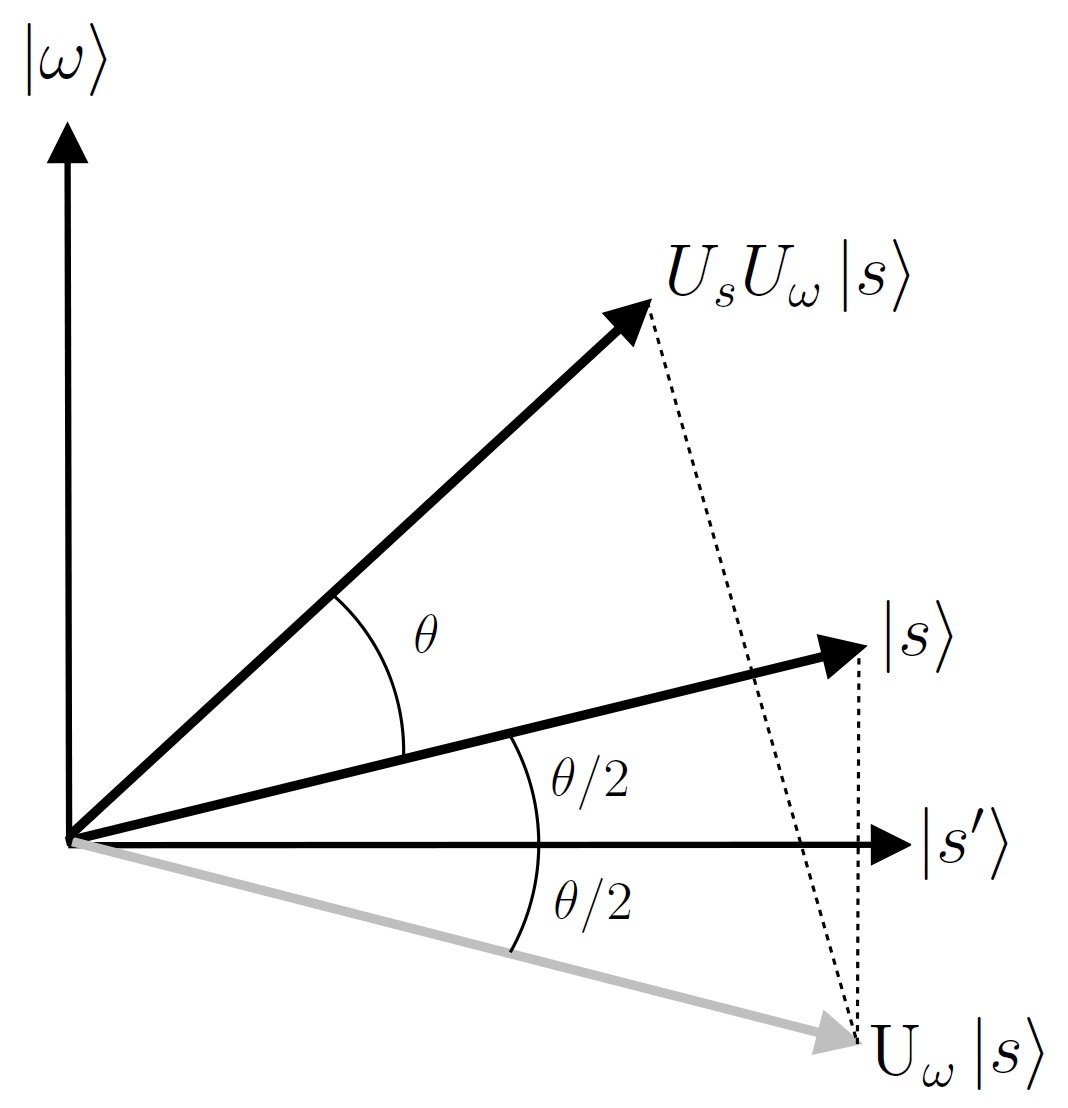
\includegraphics[width=0.3\linewidth]{../img/grover_geometry.png}
\caption{Interpretación geométrica del operador difusión}
\end{figure}

$U_s = 2 \ket{s} \bra{s} - I$

$U_{\omega} = I - 2 \ket{\omega} \bra{\omega}$

\section{El algoritmo}

\[
\Qcircuit @C=1.4em @R=1.8em {
\lstick{\ket{0}} & {/^n} \qw & \gate{H^{\otimes n}} & \multigate{1}{U_{\omega}} & \gate{U_s} & \meter & \cw \\
\lstick{\ket{1}} & \qw & \gate{H} & \ghost{U_{\omega}} & \qw & \qw & \qw \\
& & & \rstick{\hspace{-13pt} \frac{\pi}{4} \sqrt{N} \text{ veces}}
\gategroup{1}{4}{2}{5}{1.8em}{_\}}
}
\]

\begin{enumerate}
\item Inicializar el estado del sistema.
\item Aplicar la transformada de Walsh-Hadamard.
\item Realizar la iteración de Grover $\lfloor \frac{\pi}{4} \sqrt{N} \rfloor$ veces.
\begin{enumerate}
\item Aplicar $U_{\omega}$.
\item Aplicar $U_s$.
\end{enumerate}
\item Realizar la medida $\Omega$.
\end{enumerate}


\chapter{Algoritmo de Shor}
El algoritmo de Shor es un AC de factorización de enteros. Dado un entero $N=p \times q$, donde $p$ y $q$ son primos, el algoritmo de Shor encuentra $p$ y $q$ en $O((\log(N))^3)$ pasos. El algoritmo clásico más eficiente para factorizar enteros es la cibra general del cuerpo de números y funciona con una complejidad heurística de $O(e^{(\sqrt[3]{\frac{64}{9}}+o(1))(\ln(N))^{\frac{1}{3}}(\ln(\ln(N)))^{\frac{2}{3}}})$. Por su capacidad de factorizar números semiprimos, el algoritmo de Shor es capaz de violar el cifrado RSA y el protocolo Diffie-Hellman de intercambio de llaves, sobre los cuáles se basa virtualmente toda la criptografía actual.

1) Co-primos:

Dos números primos entre sí, es decir co-primos o primos relativos, son números enteros a y b que no tienen ningún factor primo en común. Es decir, sólo tienen como divisor común a 1 y -1. Esto es equivalente a decir que su máximo común divisor es 1.

Dos primos entre sí no tienen porque ser primos absolutos en forma individual.

Ejemplo:

35 | 7          6 | 3
 5 | 5          2 | 2
 1 | 1          1 | 1
 1 |            1 |

 mcd(6, 35) = 1
 pero 6 = 3.2.1 -> no es primo
 35 = 7.5.1 -> no es primo

 Estimación de orden:

 * Definición de congruencia: Dado $m \in ZZ, m \geq 1$, se dice que $a,b \in ZZ$ son congruentes módulo m si y sólo si m/(a-b).

 - Se denota por $a \equiv b mod m$, siendo m el módulo de la congruencia.
 - Si m divide a a-b, esto supone que ambos a y b tienen el mismo resto al ser divididos por el módulo m.

 Ejemplos:

 $23 \equiv 2 mod 7 \rightarrow 23 \equiv 3 7 + 2$
 $-6 \equiv 1 mod 7 \rightarrow -6 \equiv -7 1 +1$

 Además si $m \in NN$ y $a,b,c,d \in ZZ$ tales que:

 $a+c \equiv b+d mod m$
 $a c \equiv b d mod m$

 Por definición el orden $x mod N$ es el menor entero r distinto de cero que satisface $x^r = 1 mod N$
 
 Es decir:

 Sea $x = 4, N = 13 \rightarrow 4^p = 13 q + remainder ((R)); 4^p mod 13 = remainder$

 \[\begin{matrix}
         p  &   4^p & 4^p = 13 q                    + R    &   R   \\
         0  &   1   & 4^0 = 13 0                    + 1    & 1     \\
         1  &   4   & 4^1 = 13 0                    + 4    & 4     \\
         2  &   16  & 4^2 = 13 1                    + 3    & 3     \\
         3  &   64  & 4^3 = 13 4                    + 12   & 12    \\
         4  &   256  & 4^4 = 13 19                  + 9    & 9     \\
         5  &   1024  & 4^5 = 13 78                 + 10   & 10    \\ % Revisar tabla | Error en la clase
         6  &   4096  & 4^6 = 13 315                + 1    & 1     \\
         7  &   16384  & 4^7 = 13 1260              + 4    & 4     \\
         8  &   65536  & 4^8 = 13 5041              + 3    & 3     \\
         9  &   262144  & 4^9 = 13 20164            + 12   & 12    \\
         10 &   1048576  & 4^10 = 13 80659          + 9    & 9     \\
         11 &   4194304  & 4^11 = 13 322638         + 10   & 10    \\
         12 &   16777216  & 4^12 = 13 1290555       + 1    & 1     \\
         13 &   67108864  & 4^13 = 13 5162220       + 4    & 4     \\
         14 &   268435456  & 4^14 = 13 20648881     + 3    & 3     \\
         15 &   1073741824  & 4^15 = 13 82595524    + 12   & 12    \\
         16 &   4294967296  & 4^16 = 13 330382099   + 9    & 9     
     \end{matrix}
 \]

 Como podemos ver el período es r=6, el cual corresponde al menor r entero distinto de cero para el cual se cumple $4^r=1 mod 13$ con r=6

 $\therefore 4^6 = 1 mod 13$

* Expansión en fracciones contínues: (Emmanuel Desurvire -> Apéndice R)

Definamos un número real $\chi_n = a_0 \frac{1}{a_1 + \frac{1}{a_2 + \frac{1}{a_3 + \frac{1}{... a_n}}}}$ con $n \leq N$. Cada número real en el conjunto $\{x_0,x_1,...,x_{N-1},x_N\}$ se denomina un convergente de $x_n$, mientras que $x_n$ se denomina el n-ésimo convergente de $x_n$.

Propiedad 1:

El conjunto finito $\{a_0,a_1,a_2,...,a_n\}$ de números reales positivos corresponde a la razón: $x_n = \frac{p_n}{q_n}$, donde los $p_n$ y $q_n$ son definidos como:

$p_n = a_n p_{n-1} + p_{n-2}$
$q_n = a_n q_{n-1} + q_{n-2}$

con $n \geq 2, p_0 = a_0, q_0 = 1, p_1 = 1 + a_0 a_1 y q_1 = a_1$, para n = 0, 1.

Propiedad 2:

Los números reales $p_n$, $q_n$ son coprimos y satisfacen la relación:

$q_n p_{n-1} - p_n q_{n-1} = (-1)^n)$

Propiedad 3:

Dado un número racional x, si dos enteros p, q son tales que:

$|\frac{p}{q} - x| \leq \frac{1}{2q^2}$

Entonces p/q es un convergente de x.

Asumamos como ejemplo:

$\phi = 711/413 = 1.72154963680387$

Entonces:

$\phi = 711/413 = 1 + \frac{1}{1 + \frac{1}{2 + \frac{1}{1 + \frac{1}{1 + \frac{1}{2 + \frac{1}{4 + \frac{1}{5}}}}}}}$

Supongamos que solo queremos 6 decimales de precisión, es decir sea $\tilde{\phi} = 1.721549$, tal que:

$|\epsilon = |\phi - \tilde{\phi}| = 3.699 10^{-7}$

Si expandimos $\tilde{\phi}$ al igual que $\phi$, encontramos que con sólo 7 $a_n$ encontramos $\tilde{\phi}$ (ver tabla R1).

Por otro lado, $\frac{p_7}{q_7} \implies \frac{711}{413}$ da la definición de $\phi$.

* Algoritmo de factorización de Shor

El algoritmo de factorización de Shor permite factorizar números los cuales se pueden descomponer en un producto único de números primos.

Dicho número N es un entero no-primo de L bits.

En un ordenador cuántico el algoritmo de Shor tendrá un tiempo de corrida del orden $O((L^3))$ (polinómico) y en un ordenador clásico es del $O(e^[L^{1/3} (log L)^{2/3}])$ (exponencial), mostrando así que el algorimo de Shor es capaz de factorizar números muy grandes en tiempos polinómicos.

En dicho algoritmo se conjugan:

1. Aritmética modular <- Clásico
2. Paralelismo cuántico <- Cuántico
3. Transformada cuántica de Fourier <- Cuántico

El algoritmo consiste en dos etapas:

1) Una reducción del problema de descomponer en factores al problema de encontrar el orden

2) Un algoritmo cuántico para solucionar el problema de encontrar el período.

El algoritmo de Shor fue publicado en: P.W. Shor SIAM I. Comput. 26, 1484-1509 (1997(

Siguiendo el esquema de Emmanuel Desuvire "Classical and Quantum Information Theory: An Introduction for the Telecom Scientist".

La parte cuántica del algoritmo de Shor la podemos dividir en 2 partes:

1) El algoritmo de estimación de fase
2) El algoritmo de determinación de orden

Entonces:

* Estimación de fase:

Asumamos que tenemos un operador U, con autoestados $\ket{u}$ de dimensión L, y con autovalore complejos dessconocidos $\lambda_\phi = e^{2 i \pi \phi}$, donde $\phi$ es un número real tal que $0 \leq \phi \leq 1$, a ser determinado.

Asumamos también que somos capaces de construir una familia de operadores $controlled-U^p$, donde $p = 2^0, 2^1, 2^2, ..., 2^{k-1}$

El circuito cuántico del algoritmo de estimación de fase viene expresado en dos etapas, a las que llamaremos "front-end" y "back-end".

Analicemos la etapa front-end:

%%%%%% CIRCUITO AQUÍ %%%%%%

Recordemos que:

%C

Analicemos ls compuerta $CU^p \equiv controlled-U^p gate$:

%C

$U \ket{u} = e^{2 i \pi \phi}$
$U^p \ket{u} = e^{2 i \pi p \phi}$
$H \ket{0} = \ket{0} + \ket{1}$ (Sin $1\sqrt{2}$ por los momentos)

$CU^p ((\ket{0} + \ket{1}) \otimes \ket{u} = \ket{0} \otimes \ket{u} + \ket{1} \otimes U^p \ket{u} = \ket{0} \otimes \ket{u} + \ket{1} e^{2i \pi p \phi} \ket{u} = (\ket{0} + e^{2 i p \pi \phi}) \otimes \ket{u}$

$\therefore CU^p ((\ket{0} + \ket{1}) \otimes \ket{u}) = (\ket{0} + e^{2 i \pi p \phi} \ket{1}) \otimes \ket{u}$

Analicemos ahora el producto tensorial a la salida de dos compuertas $CU^p$ recordemos que $p = \{2^0, 2^1, ..., 2^{k-1}\}$, entonces:

$(\ket{0} + e^{2 i \pi 2^1 \phi} \ket{1}) \otimes (\ket{0} + e^{2 i \phi 2^0 \phi} \ket{1}) = \ket{0} \ket{0} + e^{2 i \pi 2^0 \phi} \ket{0} \ket{1} + e^{2 i \pi 2^1 p} \ket{1} \ket{0} + e^{2 \pi i (2^1 + 2^0) \phi} \ket{1} \ket{1} = e^{2 i \pi 0 \phi} \ket{0} + e^{2 i \pi 1 \phi} \ket{1} + e^{2 i \pi 2 \phi} \ket{2} + e^{2 i \pi 3 \phi} \ket{3}$

donde $\ket{00} \equiv \ket{0}; \ket{01} \equiv \ket{1}; \ket{10} \equiv \ket{2}; \ket{11} \equiv \ket{3};$

% revisar exponentes | error en la clase
es decir: $\ket{ij} \equiv \ket{i 2^0 + j 2^1}$ con i,j = 0,1
si generalizamos: $\ket{i j k ... n} = \ket{i 2^0 + j 2^1 + k 2^2 + ... + n 2^{n-1}}$

$\therefore (\ket{0} + e^{2 i \pi 2^1}) \otimes (\ket{0} + e^{2 i \pi 2^0 \phi} \ket{1}) = \sum\limits_{k = 0}^3 e^{2i \pi k \phi} \ket{k}$

Todo número puede ser representado en forma binaria:

$0 \leq \phi \leq 1 \implies \phi \equiv 0 \phi_1 \phi_2 \phi_3 ... \implies \phi = \frac{\phi_1}{2} + \frac{\phi_2}{4} + \frac{\phi_3}{8} + ... + \frac{\phi_k}{2^k} + ...$

para bits $\phi_i = 0,1 \rightarrow \phi_1 = 0 y \phi_2 = 1$

luego: .) $2^{k-1} \phi = 2^{k-1} ( \frac{\phi_1}{2} + \frac{\phi_2}{4} + \frac{\phi_3}{8} + ... + \frac{\phi_k}{2^k} + ...) = \{\phi_1 2^{k-2} + \phi_2 2^{k-3} + ... + \phi_{k-1} 2^0\} + \frac{\phi_k}{2} + \frac{\phi_{k-1}}{4} + ...$

.) $2^{k-2} \phi = 2^{k-2} ( \frac{\phi_1}{2} + \frac{\phi_2}{4} + \frac{\phi_3}{8} + ... + \frac{\phi_k}{2^k} + ...) = \{\phi_1 2^{k-3} + \phi_2 2^{k-4} + ... + \phi_{k-2} 2^0\} + \frac{\phi_{k-1}}{2} + \frac{\phi_k}{2} + \frac{\phi_{k+1}}{8} + ...$

Los términos dentro de los \{ \} son enteros. Definamos entonces:

$\Omega_m = \sum\limits_{l=1}^m \frac{\phi_{k-m+l}}{2^l}$

tal que:

$e^{2 i \pi 2^{k-1} \phi} = e^{2 i \phi \Omega_1} e^{2 i \pi (\frac{\phi_{k+1}}{4} + ...)}$
$e^{2 i \pi 2^{k-2} \phi} = e^{2 i \phi \Omega_2} e^{2 i \pi (\frac{\phi_{k+1}}{8} + ...)}$
.
.
.
$e^{2 i \pi 2^0 \phi} = e^{2 i \phi \Omega_k} e^{2 i \pi (\frac{\phi_{k+1}}{2^{k+1}} + ...)}$

Consideremos el caso en el cual $\phi$ es definido exactamente por k bits tal que $\phi_{k+1} = \phi_{k+2} = ... = 0$

Dejando de lado el qubit $\ket{u}$ la salida del primer registro es:

$\frac{1}{2^{k/2}} (\ket{0} + e^{2 i \pi \Omega_1} \ket{1}) \otimes (\ket{0} + e^{2 i \pi \Omega_2}) \otimes ... \otimes (\ket{0} + e^{2 i \pi \Omega_k} \ket{1})$

Como podemos recordar

$QFT \ket{n} = \frac{1}{2^{k/2}} (\ket{0}_1 + e^{2 i \pi \Omega_1} \ket{1}_1) \otimes (\ket{0}_2 +  e^{2 i \pi \Omega_2} \ket{1}_2) \otimes ... \otimes (\ket{0}_k + e^{2 i \pi \Omega_k} \ket{1}_k)$

Siendo: $1 \leq m \leq k \rightarrow \ket{m} = \frac{1}{2^{m/2}} (\ket{0}_m + e^{2 i \pi \Omega_m} \ket{1}_m)$

con $\Omega_m = \sum\limits_{l=1}^m \frac{n_{k-m+l}}{2}$

Encontrando así que $\frac{1}{2^{k/2}} (\ket{0} + e^{2 i \pi \Omega_1} \ket{1}) \otimes (\ket{0} + e^{2 i \pi \Omega_2} \ket{1}) \otimes ... \otimes (\ket{0} + e^{2 i \pi \Omega_k} \ket{1})$

Es la transformada cuántica de Fourier de nuestro estado $\ket{\phi}$ obtenida con las compuertas $Controlled-U^p$.

Al ket $\ket{\phi}$ lo podemos recuperar haciendo la transformada inversa de Fourier.

Consideremos ahora el módulo del circuito cuántico "back-end"

% C

El módulo back-end del circuito cuántico de Shor consiste en realizar la transformada cuántica inversa de Fourier y hacer medidas sobre los k qubits encontrando así los $\phi_1, \phi_2,...,\phi_k$.

Seguidamente consideremos ahora el caso más general en el cual $2^k \phi$ no es un entero.

Fron-end $\ket{0}^{\otimes k} \otimes \ket{u} \rightarrow \frac{1}{\sqrt{N}} \sum\limits_{k=0}^{N-1} e^{2 i \pi k \phi} \ket{k} \otimes \ket{u}$

Back-end $QFT_1^\dagger (\frac{1}{\sqrt{N}} \sum\limits_{k=0}^{N-1} e^{2 i \pi k \phi} \ket{k} \otimes \ket{u}) = \frac{1}{\sqrt{N}} \sum\limits_{k=0}^{N-1} e^{2 i k \phi} QFT^\dagger \ket{k} \otimes \ket{u} = \frac{1}{\sqrt{N}} \sum\limits_{k=0}^{N-1} e^{2 i \pi k \phi} (\frac{1}{2^{k/2}} \sum\limits_{n=0}^{N-1} e^{-\frac{2 \pi i k n}{N} \ket{n}) \ket{u} = \frac{1}{N} \sum\limits_{k=0}^{N-1} \sum\limits_{n=0}^{N-1} e^{- 2 \pi i \frac{k n}{N}} e^2 i pi k \phi} \ket{n} \otimes \ket{u} = \frac{1}{N} \sum\limits_{n=0}^{N-1} (\sum\limits_{k=0}^{N-1} (e^{2 i \pi (\phi - \frac{n}{N})})^k ) \ket{n} \otimes \ket{u}$

$\therefore (QFT^\dagger \otimes \mathds{1}) (\frac{1}{\sqrt{N}} \sum\limits_{k=0}^{N-1} e^{2 i \pi k \phi} \ket{k} \otimes \ket{u}) = \frac{1}{N} \sum\limits_{n=0}^{N-1} (\frac{1 - e^{2 i \pi (\phi - \frac{n}{N})N}}{1 - e^{2 i \pi (\phi - \frac{n}{N})}}) \ket{n} \otimes \ket{u}$

La probabilidad de medir n a la salida del registro será:

$p(n) = |\bra{u} \otimes \bra{n} \ket{\psi_{output}}|^2$

$p(n) = \frac{1}{N^2} |\frac{1 - e^{2 i \pi (\phi - \frac{n}{N})N}}{1 - e^{2 i \pi (\phi - \frac{n}{N})}}|^2$

$\therefore p(n) = \frac{1}{N^2} \frac{\sin^2(\pi (\phi - \frac{n}{N}) N)}{\sin^2(\pi (\phi - \frac{n}{N}))}$

La medida de n con probabilidad asociada p(n), corresponde a la estimación de fase $\tilde{\phi} = n/N$. La probabilidad es máxima cuando $\delta = \phi - \tilde{\phi}$ es mínima.

$p(n) = \frac{1}{N^2} \frac{\sin^2(\pi (\phi - \frac{n}{N}) N)}{\sin^2(\pi (\phi - \frac{n}{N}))}$ si N es grande $\rightarrow$ %Graf

La probabilidad p(n) decae rápidamente a cero cuando el error $\delta$ se aleja del mínimo.

Entonces:

.) La medida tiene la maor probabilidad de dar la aproximación más cercana al estado $\phi$.
.) El circuito de salida es de la forma $\ket{\tilde{\phi}} \ket{u}$, donde $\ket{\tilde{\phi}}$ es una superposición de estados, los cuales al medirlos dan una buena aproximación de $\phi$.

* Estimación de orden:

Analicemos como la estimación de fase hace posible determinr r, el orden de x mod N, con alta probabilidad y precisión.

Primero necesitamos introducir el operador U y sus correspondientes autovectores y autovalores.

Asumamos que dados dos enteros x y N que satisfacen que x<N, siendo x coprimo de M, es decir mcd(x,M)=1, existe un operador $U_{x,N}$ que actúa sobre el qubit $\ket{y} \equiv \{\ket{0}, \ket{1}\}$, tal que:

$U_{x,N} \ket{y} = \ket{x y mod N}$

Asumamos $\{ \ket{u_s}\}_{s = 0, 1, ..., r-1}$ el conjunto de r autoestados de U, asociados con los autovalores $e^{i 2 \pi s/r}$ tal que $U \ket{u_s} = e^{2 i \pi s /r} \ket{u_s}$ en el cual la fase es $\phi_s = s/r$ con $0 \leq \phi_s \leq 1$

Tales autoestados $\ket{u_s}$ se definen acorde a: $\ket{u_s} = \frac{1}{\sqrt{r}} \sum\limits_{k=0}^{r-1} e^{\frac{-2 i \pi k s}{r}} \ket{x^k mod N}$, siendo r a determinar.

Con las siguientes propiedades:

$\frac{1}{\sqrt{r}} \sum_{s=0}{r-1} \ket{u_s} = \ket{1}$

$\frac{1}{\sqrt{r}} \sum\limits_{s=0}^{r-1} e^{\frac{2 i \pi k s}{r}} \ket{u_s} = \ket{x^k mod N}$

$p(s) = |c_s|^2 = \frac{1}{r}$

El circuito para la estimación de orden es el siguiente:

%%%%%% Circuito aqui%%%%%%

Entonces:

$U_{x,y} \ket{y} = \ket{x y mod N}$

$j = 2^0, 2^1, 2^2, ..., 2^{k-1}$

$CU^j (\ket{0} \otimes \ket{1}) = \ket{0} \otimes \ket{1}$

$CU^j \ket{j} \otimes \ket{1} = \ket{j} \otimes \ket{x^{j_1 2^{k-1}} mod N} \ket{x^{j_2 2^{k-2}} mod N} ... \ket{x^{j_k 2^0} mod N}$

$CU^j \ket{j} \otimes \ket{1} = \ket{j} \otimes \ket{x^{j_1 2^k-1} x^{j_2 2^{k-2}} ... x^{j_k 2^0} mod N}$

$\therefore CU^j \ket{j} \otimes \ket{1} = \ket{j} \otimes \ket{x^j mod N}$

Con este paso entendido vamos ahora a analizar el circuito para determinar el orden:

1) $\ket{\psi_1} = \ket{0}^{\otimes k} \otimes \ket{1}$

2) $\ket{psi_2} = \frac{1}{\sqrt{M}} (\ket{0} + \ket{1})^{\otimes k} \otimes \ket{1}; M=2^k$

$\ket{psi_2} = \frac{1}{\sqrt{M}} \sum_{j=0}^{M-1} CU^j (\ket{j} \otimes \ket{1})$

3) $\ket{\psi_3} = CU^j \ket{\psi_2} = \frac{1}{\sqrt{M}} \sum\limits_{j=0}^{M-1} CU^j (\ket{j} \otimes \ket{1}) = \frac{1}{\sqrt{M}} \sum\limits_{j=0}^{M-1} (\ket{j} \otimes \ket{x^j mod N})$

Pero ya vimos que: $\ket{x^j mod N} = \frac{1}{\sqrt{r}} \sum\limits_{s=0}^{r-1} e^{\frac{2 i \pi k s}{r}} \ket{u_s}$

$\therefore \ket{\psi_3} = \frac{1}{\sqrt{M}} \sum\limits_{k=0}^{M-1} \ket{k} \otimes \frac{1}{\sqrt{r}} e^{2 i \pi k s/r} \ket{u_s}$

$\ket{\psi_3} = \sum\limits_{s=0}^{r-1} (\frac{1}{\sqrt{M}} \sum_{k=0}^{M-1} e^{2 i \pi k s/r} \ket{k}) \otimes \frac{1}{\sqrt{r}} \ket{u_s}$

4) Aplicamos la transformada inversa de Fourier al primer registro $\ket{\psi_4} = (QFT^\dagger \otimes \mathds{1}) \ket{\psi_3} = \frac{1}{\sqrt{r}} \sum\limits_{s=0}^{r-1} \ket{\tilde{\psi}_s} \otimes \ket{u_s}$

Finalmente: Al medir el primer registro proyectamos la superposición que conforma $\ket{\psi_4}$ en uno de los r estados de $\ket{\psi_s}$

$p(s) = |(\bra{\tilde{\psi}_s} \otimes \bra{u_s}) \ket{\psi_4}|^2 = \frac{1}{r}$

lo que nos da $\frac{s}{r}$ correspondiendo a la estimación de fase $\tilde{\psi} = \frac{s}{r}$

Posteriormente aplicamos el algoritmo clásico de fracciones continuas y determinamos los co-primos.

Ejemplo:

Determinemos la factorización para N=15.

Asumamos, el número compuesto N=15 (no primo). Tomemos L = log2 N = 9 para el segundo registro (tamaño del target) y pongamos un error de probabilidad grande $\epsilon = 0.25$.

$k = 2L + 1 + \log_2(2 + \frac{1}{2 \varepsilon} = 11$ (ver libro: tamaño del primer registro de control)

$M = 2^k = 2^{11} = 2048$

tomemos un número x aleatorio entre $[2, N-1] \rightarrow x = 8$ lo cual cumple que m.c.d(8,15) = 1

Pasos cuánticos:

.) $\ket{\psi_1} = \ket{0}^{\otimes k} \otimes \ket{1}$

.) $\ket{\psi_2} = \frac{1}{\sqrt{M}} \sum\limits_{j=0}^{M-1} (\ket{j} \otimes \ket{1}) = \frac{1}{\sqrt{2^M}} (\ket{0} + \ket{1} + \ket{2} + ... + \ket{M-1})$

.) Aplicamos la compuerta $Controlled-U^j$ $\ket{\psi_3} = \frac{1}{\sqrt{M}} \ket{j} \otimes \ket{x^j mod N} = \frac{1}{\sqrt{M}} \sum\limits_{j=0}^{M-1} \ket{1} \otimes \ket{8^j mod 15}$

$\ket{\psi_3} = \frac{1}{\sqrt{M}} (\ket{0}\ket{1} + \ket{1}\ket{8} + \ket{2}\ket{4} + \ket{3}\ket{2} + \ket{4}\ket{1} + \ket{5}\ket{8} + \ket{6}\ket{4} + \ket{7}\ket{2} + \ket{8}\ket{1} + \ket{9}\ket{8} + \ket{0}\ket{4} + \ket{1}\ket{2} + ...)$

$\ket{\psi_3} = \frac{1}{\sqrt{M}} ((\ket{0} + \ket{4} + \ket{8} + ...)\ket{1} + (\ket{1} + \ket{5} + \ket{9} + ...) \ket{8} + (\ket{2} + \ket{6} + \ket{10} + ...) \ket{4} + (\ket{3} + \ket{7} + \ket{11} + ...) \ket{2})$

Definamos: $\ket{u_1} = \frac{1}{\sqrt{M}} (\ket{0} + \ket{4} + \ket{8} + ...)$

$\ket{u_2} = \frac{1}{\sqrt{M}} (\ket{1} + \ket{5} + \ket{9} + ...)$

$\ket{u_3} = \frac{1}{\sqrt{M}} (\ket{2} + \ket{6} + \ket{10} + ...)$

$\ket{u_4} = \frac{1}{\sqrt{M}} (\ket{3} + \ket{7} + \ket{11} + ...)$

y obtenemos: $\ket{\psi_3} = \ket{u_1} \otimes \ket{1} + \ket{u_2} \otimes \ket{8} + \ket{u_3} \otimes \ket{4} + \ket{u_4} \otimes \ket{2}$

Consideremos el primer registro $\ket{u_2} \otimes \ket{8}$, es decir $\ket{u_2}$, y apliquemos la $QFT^\dagger$ sobre él.

$QFT^\dagger \ket{u_2} = \frac{1}{\sqrt{M}} QFT^\dagger (\ket{1} + \ket{5} + \ket{9} + \ket{13} + ...)$

Recordemos que $QFT^\dagger \ket{n} = \frac{1}{\sqrt{4 M}} \sum\limits_{k=0}^{M-1} e^{-2 i \pi k n /M} \ket{k}$

Luego: $QFT^\dagger \ket{u_2} = \frac{1}{\sqrt{M}} QFT^\dagger (\ket{1} + \ket{5} + \ket{9} + \ket{13} + ...)$

$QFT^\dagger \ket{u_2} = \frac{1}{2M} \sum\limits_{k=0}^{M-1} (e^{- \frac{k 2 i \pi}{M} 1} \ket{k} + e^{- \frac{k 2 i \pi}{M} 5} \ket{k} + e^{- \frac{k 2 i \pi}{M} 9} \ket{k} + e^{- \frac{k 2 i \pi}{M} 13} \ket{k} + ...)$


$QFT^\dagger \ket{u_2} = \frac{1}{2M} \sum\limits_{k=0}^{M-1} (e^{- \frac{k 2 i \pi}{M} 1} + e^{- \frac{k 2 i \pi}{M} 5} + e^{- \frac{k 2 i \pi}{M} 9} + e^{- \frac{k 2 i \pi}{M} 13} + ...) \ket{k}$

$QFT^\dagger \ket{u_2} = \frac{1}{2M} \sum\limits_{k=0}^{M-1} e^{- \frac{k 2 i \pi}{M} 1} ((e^{- \frac{k 8 i \pi}{M}})^0 + (e^{- \frac{k 8 i \pi}{M}})^1 + (e^{- \frac{k 8 i \pi}{M}})^2 + ...) \ket{k}$

$QFT^\dagger \ket{u_2} = \frac{1}{2M} \sum\limits_{k=0}^{M-1} e^{-k \frac{2 i \pi}{M}} \sum\limits_{m=0}^{M-1} (e^{-k \frac{8 i \pi}{M}})^m \ket{m}$

$QFT^\dagger \sum\limits_{k=0}^{M-1} e^{-k \frac{2 i \pi}{M}} \frac{(1-e^{-8 i \pi k})}{(1 - e^{-k \frac{8 i \pi}{M}})} \ket{k}$

$QFT^\dagger \ket{u_2} = \frac{1}{2M} \sum_{k=0}^{M-1} e^{-k \frac{2 \pi i}{M}} \frac{(1 - e^{-8 i \pi k}}{e^{-k \frac{4 i \pi}{M}} (e^{k \frac{4 i \pi}{M}} - e^{-k \frac{4 i \pi}{M}})} \ket{k}$

$QFT^\dagger \ket{u_2} = \frac{1}{4 i M} \sum_{k=0}^{M-1} e^{k \frac{2 \pi i}{M}} \frac{(1 - e^{-8 i \pi k})}{\sin(\frac{4\pi k}{M})} \ket{k}$

$QFT^\dagger \ket{u_2} = \frac{1}{4 i M} \sum_{k=0}^{M-1} e^{k \frac{2 \pi i}{M}} \frac{e^{-4 i \pi k} (e^{4 i \pi k} - e^{-4 i \pi k})}{\sin(\frac{4\pi k}{M})} \ket{k}$

$QFT^\dagger \ket{u_2} = \frac{1}{2M} \sum_{k=0}^{M-1} e^{-k \frac{2 \pi i}{M} (2M-1)} \frac{\sin(4\pi k)}{\sin(\frac{4\pi k}{M})} \ket{k}$

Este resultado se puede reescribir de la forma:

$QFT^\dagger \ket{u_2} = \sum\limits_{k=0}^{M-1} \alpha_k \ket{k}$

siendo $\alpha_k = \frac{1}{2M} e^{-k \frac{2 i \pi}{M} (2M-1)} \frac{\sin(4 \pi k)}{\sin(k \frac{4 \pi}{M})}$

correspondiendo $p(k) = |\bra{k} QFT^\dagger \ket{u_2}|^2 = |\alpha_k|^2 = \frac{1}{4M^2} \frac{\sin^(4\pi k)}{\sin^2(\frac{4 \pi k}{M})}$

Como podemos observar para todo entero k=0,1,...,M-1 el número de $\alpha_k$ es cero, pero para $\frac{4 \pi k}{M} = n \pi \rightarrow k = n \frac{M}{4} = n 2^7 = n 512$, n entero

el denominador es cero y $\alpha_k$ es indeterminado, luego:

$\lim_{\epsilon \to 0} \frac{\sin^2(4 \pi k)}{\sin^2(\frac{4\pi k}{M})} = \lim_{\epsilon \to 0} \frac{\sin^2(4 \pi (\frac{n M}{4} + \epsilon))}{\sin^2(\frac{4\pi}{M} (\frac{n M}{4} + \epsilon))} = \lim_{\epsilon \to 0} \frac{\sin^2(n M \pi + 4 \pi \epsilon)}{\sin^2(n \pi + \frac{4\pi}{M} \epsilon} = \lim_{\epsilon \to 0} \frac{\sin^2(4 \pi \epsilon)}{\sin^2(\frac{4 \pi}{M} \epsilon)} = \frac{(4 \pi \epsilon)}{(\frac{4 \pi}{M} \epsilon)^2} = M^2$

luego: $p(k)_{\text{Máximo}} = \frac{1}{4M^2} M^2 \rightarrow p_{Maximo}(k) = \frac{1}{4}$

En el rango k=0,1,...,M-1 los máximos de p(k) están localizados en:

$k=0 \rightarrow n=0$
$k=512 \rightarrow n=1$
$k=1024 \rightarrow n=2$
$k=1536 \rightarrow n=3$

%%%%%%%%%% Grafico aqui %%%%%%%%%%%

Al medir obtenemos: $\frac{k_i}{M} = \frac{k_i}{2^k} = \frac{k_i}{2^{13}} = \frac{k_i}{2048}$

las cuatro posibles determinaciones de $\tilde{\phi}$ son:

$\left. \frac{0}{2048} \right|_{k_i=0}; \left. \frac{512}{2048} \right|_{k_i=512}; \left. \frac{1024}{2048} \right|_{k_i=1024}; \left. \frac{1536}{2048} \right|_{k_i=1536};$

$k_i = 0$ no aporta nada
$k_1 = \frac{512}{2048} = \frac{1}{4}$ \} no satisfacen $|\frac{s}{r} - x| \leq \frac{1}{r^2}$
$k_2 = \frac{1024}{2048} = \frac{1}{2}$ \} no satisfacen $|\frac{s}{r} - x| \leq \frac{1}{r^2}$
$k_3 = \frac{1536}{2048} = \frac{1}{1+\frac{1}{3}}$

ya que $\frac{p_0}{1_0} = \frac{0}{1}; \frac{p_1}{q_1} = \frac{1}{1}; \frac{p_2}{q_2} = \frac{3}{4}$

3 y 4 son co-primos.

La fracción 3/4 es un convergente de $\phi$ y $r = q_2 = 4$ es el orden de x

Normalmente se suele asociar con que existen 2 $N^\prime$ y $N^{\prime\prime}$ de N=15 tales que

$N^\prime = MCD(x^{r/2} - 1, N) = MCD(63, 15) = 3$
$N^{\prime\prime} = MCD(x^{r/2} + 1, N) = MCD(65, 15) = 5$













%aqui%










\section{Transformadas integrales}

\section{Transformada cuántica de Fourier}

\section{Estimación de fase}

\section{Estimación de orden}

\section{Algoritmo de Shor}

\chapter{Google PageRank}
% El PageRank, nombrado en honor a Larry Page, es una de las medidas de centralidad de los nodos de un grafo más conocidas. Ésta es utilizada para ordenar los sitios web en los resultados de búsqueda de Google, de acuerdo a su importancia.

El algoritmo de PageRank fue desarrollado en 1996 en la Universidad de Stanford por Larry Page y Sergey Brin, los cuales fueron los fundadores de Google.

Este algoritmo se basa en la idea de que sitios web importantes tienen muchos vínculos que apuntan hacia ellos, lo que conduce a pensar en la web como una red ponderada orientada.

Existen muchos otros algoritmos, algunos más eficientes, pero la importancia de PageRank se sustenta en el poder económico de Google.

Ilustraremos el algoritmo de PageRank con un ejemplo sencillo:

Ejemplo:

Consideremos 5 páginas web distintas a las que denotaremos por 1, 2, 3, 4, y 5, y cuyo grafo es:

Pasos:
\begin{enumerate}
\item Determinar la matriz de adyacencia. Algunos autores denotan la matriz de de adyacencia por M en el protocolo de PageRank

\[
M = \begin{pmatrix}
0 & 0 & 1 & 1 & 1 \\
0 & 0 & 0 & 0 & 1 \\
1 & 0 & 0 & 1 & 1 \\
1 & 0 & 1 & 0 & 0 \\
1 & 1 & 0 & 0 & 0
\end{pmatrix}
\]

\item Sumamos los elementos de cada una de las columnas.

\[
\begin{matrix}
3 & 1 & 2 & 2 & 3
\end{matrix}
\]

Estas sumas representan el número de links que salen del nodo o vértice de la página $p_j$, es decir: 

$I(p_j) \equiv \text{Importancia de la página j}$

$\mathrm{outdeg}(p_j) \equiv \text{número de links que salen de la página } p_j$

$I(p_i) \equiv \sum\limits_{j \in B_i} \frac{I(p_j}{\mathrm{outdeg}(p_j)}$

$B_i \equiv \text{conjunto de páginas qeu son linkeadas}$

\item Dividimos cada elemento de M por la suma de los elementos de la columna a la cual corresponde y llamaremos a la nueva matriz obtenida $M^\prime$

\[
M^\prime = \begin{pmatrix}
0 & 0 & 1/2 & 1/2 & 1/3 \\
0 & 0 & 0 & 0 & 1/3 \\
1/3 & 0 & 0 & 1/2 & 1/3 \\
1/3 & 0 & 1/2 & 0 & 0 \\
1/3 & 1 & 0 & 0 & 0
\end{pmatrix}
\]

\item El siguiente paso es encontrar un vector $\vec{v}$ (algunos autores lo llaman $\vec{I}$) que represente el PageRank de cada una de las páginas. Como tenemos 5 páginas web le asignamos a $\vec{v}$ como valores $\vec{v} = (a,b,c,d,e)^T$, obteniendo así un vector de dimensión $d=5$.

\item Obtenemos los valores de $\{v_i\}$ a partir de los autovalores de $M^\prime$, tal que:

\[
M^\prime \vec{v} = \lambda \vec{v} \text{ con }\lambda \in R
\]

\item Determinamos los autovalores de $M^\prime$

\[
\lambda_1 = 1; \quad \lambda_2 = \frac{-2}{3}; \quad \lambda_3 = \frac{-1}{2}; \quad \lambda_4 = \frac{-1}{3}; \quad \lambda_5 = \frac{1}{3}
\]

Tomaremos sólo $\lambda = 1$ $\rightarrow M^\prime \vec{v} = \vec{v}$ (Ecuación autoconsistente)

\item Hallamos el autovector asociado a $\lambda = 1$. Obteniendo:

\[
a = 6; \quad b = 1; \quad c = \frac{16}{3}; \quad d = \frac{14}{3}; \quad e = 3
\]

\item Finalmente, Google ordena de mayor a menor las componentes de $\vec{v}$, quedándonos:

\[
\begin{matrix}
& & - & a \\
& & - & c \\
\text{Pantalla} & \rightarrow & - & d \\
& & - & e \\
& & - & b
\end{matrix}
\]
\end{enumerate}

La idea de PageRank de Google es que la importancia de una página viene dada por la cantidad de páginas que se enlazan con ella.

Surgen varios problemas:

\begin{enumerate}
  \item Las matrices hyperlink (hiperenlace) pueden tener billones de entradas en filas y columnas.
  \item Calcular los autovectores es un absurdo computacional.
  \item Los estudios muestran que un nodo (página web) tiene un promedio de 10 enlaces, y las demás entradas de la matriz son cero.
  \item No se encuentra $\lambda = 1$ en la mayoría de los casos.
\end{enumerate}

Por esta razón, un remedio (Patching) del algoritmo de PageRank fue el método de las potencias, en el cual la matriz hiperenlace

\[
H_{ij} \equiv \begin{cases}
\frac{1}{\mathrm{outdeg}(P_j)} & \text{si } P_j \in B_i \\
0 & \text{en otro caso}
\end{cases}
\]

debería converger a una solución autoconsistente

\[
I^{k+1} = H I^k
\]

donde se toma un vector $I^{0}$ y se hace interactuar unas 100 veces y el orden mostrado de las páginas es el de $I^{100}$, ordenadas de mayor a menor. Si se normalizan las columnas de la matriz hipervínculo (hiperenlace) $H$, obtenemos otra matriz hiperenlace normalizada E.

\textbf{La matriz E:} se sabe de la teoría de matrices estocásticas que 1 es uno de sus autovalores. Además, también se sabe que la convergencia de $I^k = E I^{k-1}$ a $I = E I$ depende del segundo autovalor de $\lambda_2$ de E y es un hecho que $I^k = E I^{k-1}$ converge rápidamente si $\abs{\lambda_2}$ es
cercano a cero.

\subsection{El algoritmo de remiendo (parcheo) general}

Asumamos que el caminante recorre el grafo siguiendo la web con una matriz estocástica E con probabilidad $\alpha$, y con probabilidad $1-\alpha$ podrá ir a cualquier página al azar que sea de su interés. La matriz web de este proceso será:

\[
G \equiv \alpha E + \frac{1-\alpha}{N} \mathds{I} \text{Matriz de Google}
\]

$\mathds{I}$ es una matriz en la cual todas las entradas están establecidas en 1, y N el número de nodos.

Propiedades de G:
\begin{enumerate}
\item Es estocástica
\item Irreducible
\item Primitiva
\item El resultado de determinar el estado auto-consistente no depende del vector Google inicial $I^0$
\end{enumerate}

\begin{figure}[H]
\begin{center}
\begin{tabular}{c c c}
 \begin{tikzpicture}[->,>=stealth',shorten >=1pt,thick]
\tikzset{VertexStyle/.style = {draw,circle,thick,
                               minimum size=0.5cm,
                               font=\bfseries},thick} 
\Vertex[a = 90, d = 2.75]{1}  \Vertex[a = 162, d = 2.75]{2}
\Vertex[a = 234, d = 2.75]{3} \Vertex[a = 306, d = 2.75]{4}
\Vertex[a = 18, d = 2.75]{5}
\Edge[label=$1$](2)(1)
\Edge[label=$1$](1)(5)
\Edge[label=$\frac{1}{2}$](3)(1)
\Edge[label=$\frac{1}{2}$](3)(4)
\Edge[label=$1$](4)(5)
\tikzset{EdgeStyle/.style = {->, bend left}}
\Edge[label=$1$](1)(3)
\end{tikzpicture} 
& \begin{tikzpicture}[->,>=stealth',shorten >=1pt,thick]
\tikzset{VertexStyle/.style = {draw,circle,thick,
                               minimum size=0.5cm,
                               font=\bfseries},thick} 
\Vertex[a = 90, d = 2.75]{1}  \Vertex[a = 162, d = 2.75]{2}
\Vertex[a = 234, d = 2.75]{3} \Vertex[a = 306, d = 2.75]{4}
\Vertex[a = 18, d = 2.75]{5}
\Edge[label=$\frac{1}{10}$](5)(4)
\Edge[label=$\frac{1}{10}$](4)(3)
\Edge[label=$\frac{1}{10}$](3)(2)
\Edge[label=$\frac{3}{5}$](2)(1)
\Edge[label=$\frac{3}{5}$](1)(5)
\Edge[label=$\frac{1}{10}$](1)(4)
\Edge[label=$\frac{1}{10}$](4)(2)
\Edge[label=$\frac{1}{10}$](2)(5)
\Edge[label=$\frac{1}{10}$](5)(3)
\Edge[label=$\frac{7}{20}$](3)(1)
\Loop[dist=1cm,dir=NO,label=$\frac{1}{10}$,labelstyle=above](1)  
\Loop[dist=1cm,dir=NOWE,label=$\frac{1}{10}$,labelstyle=above left](2)  
\Loop[dist=1cm,dir=SOWE,label=$\frac{1}{10}$,labelstyle=below left](3)  
\Loop[dist=1cm,dir=SOEA,label=$\frac{1}{10}$,labelstyle=below right](4)  
\Loop[dist=1cm,dir=NOEA,label=$\frac{1}{10}$,labelstyle=above right](5)  
\tikzset{EdgeStyle/.style = {->, bend right}}
\Edge[label=$\frac{1}{10}$,labelstyle=above left](1)(2)
\Edge[label=$\frac{1}{10}$,labelstyle=below left](2)(3)
\Edge[label=$\frac{7}{20}$,labelstyle=below](3)(4)
\Edge[label=$\frac{3}{5}$,labelstyle=below right](4)(5)
\Edge[label=$\frac{1}{10}$,labelstyle=above right](5)(1)
\Edge[label=$\frac{3}{5}$](1)(3)
\Edge[label=$\frac{1}{10}$](3)(5)
\Edge[label=$\frac{1}{10}$](5)(2)
\Edge[label=$\frac{1}{10}$](2)(4)
\Edge[label=$\frac{1}{10}$](4)(1)
\end{tikzpicture} 
 \\
(a) & (b)
\end{tabular}
\caption{Grafo correspondiente a la matriz de adyacencia (a) de la red E (b) remendada de Google G con $\alpha=\frac{1}{2}$}
\end{center}
\end{figure}


\subsection{Interpretación como una caminata aleatoria}

La asiganación de valores de importancia se puede replantear como la probabilidad de encontrar un caminante aleatorio en cierto nodo del grafo.

\begin{minipage}{0.5\linewidth}
Del proceso:
\begin{align*}
& Pr(x^{(n+1)}=p_i) \\
& =\sum\limits_j G_{i j} Pr(x^{(n)}=p_j)
\end{align*}
\end{minipage}
\begin{minipage}{0.5\linewidth}
De la ley de probabilidad total:
\begin{align*}
& Pr(x^{(n+1)}=p_i) \\
& =\sum\limits_j Pr(x^{(n+1)}=p_i|x^{(n)}=p_j) Pr(x^{(n)}=p_j)
\end{align*}
\end{minipage}
\[
\implies G_{i j} = Pr(x^{(n+1)}=p_i | x^{(n)}=p_j)
\]

En el contexto del Internet, $G_{i j}$ es la probabilidad de que cierto internauta, que se encuentra en la página $p_i$, entre en la página $p_j$. El factor $\alpha E_{i j}$ es la probabilidad de que lo haga presionando un enlace presente en $p_i$, mientras que $\frac{1-\alpha}{N} \mathds{I}$ es la probabilidad de que lo haga introduciendo la URL directamente.

El factor de amortiguamiento es libre y debe ser calibrado. Se suela usar $\alpha = 0.85$

\subsection{Cuantizando las caminatas aleatorias}

La forma obvia y directa de cuantizar una caminata aleatoria sería sustituir el conjunto de nodos $\{p_i\}$ por el conjunto de kets $\{\ket{i}\}$. Sin embargo, esto lleva a sistemas con operadores no unitarios y no es realizable.

% INSERTAR EJEMPLO AQUÍ
\begin{figure}[H]
\begin{tabular}{c c}
\begin{tikzpicture}[,>=stealth',shorten >=1pt,thick]
\tikzset{VertexStyle/.style = {draw,circle,thick,
                               minimum size=1cm,
                               font=\bfseries},thick} 
\Vertex[x = -2.2, y = 0]{-2}  \Vertex[x = -1.1, y = 0]{-1}
\Vertex[x = 0, y = 0]{0} \Vertex[x = 1.1, y = 0]{1}
\Vertex[x = 2.2, y = 0]{2}
\Edges(-2,-1,0,1,2)
\end{tikzpicture} &
\begin{tikzpicture}[,>=stealth',shorten >=1pt,thick]
\tikzset{VertexStyle/.style = {draw,circle,thick,
                               minimum size=1cm,
                               font=\scriptsize\bfseries},thick} 
\Vertex[x = -2.2, y = 0, L = $\ket{-2}$]{-2}  \Vertex[x = -1.1, y = 0, L = $\ket{-1}$]{-1}
\Vertex[x = 0, y = 0, L = $\ket{0}$]{0} \Vertex[x = 1.1, y = 0, L = $\ket{1}$]{1}
\Vertex[x = 2.2, y = 0, L = $\ket{2}$]{2}
\Edges(-2,-1,0,1,2)
\end{tikzpicture}
\end{tabular}
\end{figure}

Esto nos obliga a buscar maneras alternativas de cuantizar las caminatas aleatorias. La cadena anterior se podría cuantizar agregando un espacio "moneda" al espacio de Hilbert generado por $\{\ket{i}\}$. En este caso, el operador de difusión se interpreta como "lanzar la moneda" para decidir en qué dirección ir.

\begin{align*}
U = \sqrt{p} \ketbra{i+1}{i} \otimes \ketbra{c}{c} + \sqrt{1-p}
\ketbra{i-p}{i} \otimes \ketbra{s}{s} \\
U^\dagger = \sqrt{p} \ketbra{i}{i+1} \otimes \ketbra{c}{c} + \sqrt{1-p}
\ketbra{i}{i-p} \otimes \ketbra{s}{s} \\
U U^\dagger = p \ketbra{i+1}{i+1} \otimes \ketbra{c}{c} + (1-p) \ketbra{i-1}{i-1} \otimes \ketbra{s}{s}
\end{align*}

Al realizar la suma sobre $i$ se tiene $\mathds{1}$, como se deseaba. Sin embargo, esta solución toavía no es satisfactoria, pues exige que $p_{i j}=\frac{1}{outdeg(j)}$ para que $U U^\dagger=\mathds{1}$.

Casi todas las cuantizaciones cometen estos dos pecados, aumentar la dimensión del espacio de Hilbert e imponer condiciones sobre el grafo; y en general, se debe cometer al menos uno de los dos.

\textbf{Nota:} También existen caminatas cuánticas continuas, no sólo discretas.

\subsection{Caminata cuántica de Szegedy}

Existe un tipo particular de caminatas aleatorias conocido como caminatas bipartitas. En éstas se tiene dos conjuntos de nodos y sólo ocurren transiciones entre los dos conjuntos, no dentro del mismo.

% INSERTAR EJEMPLO AQUÍ

Szegedy desarrolló una cuantización de estas caminatas. Para esto utilizó operadores de reflexión ($W = \mathds{1} - 2 \ketbra{w}{w}$, similares a los utilizados en el algoritmo de Grover). Aprovechándose del hecho de que un par de reflexiones equivale a una rotación (como en el algoritmo de Grover), creó el siguiente operador de evolución de la caminata: $U = (\mathds{1} - 2 B)(\mathds{1} - 2 A)$, donde A es el proyector sobre las transiciones de la primera partición a la segunda y B de la segunda a la primera.

\begin{minipage}{0.5\linewidth}
\begin{align*}
\ket{\psi_i} &= \ket{i}_1 \otimes \sum\limits_j \sqrt{p_{j i}} \ket{j}_2 \\
A &= \sum\limits_i \ketbra{\psi_i}{\psi_i}
\end{align*}
\end{minipage}
\begin{minipage}{0.5\linewidth}
\begin{align*}
\ket{\psi_i} &= \sum\limits_i \sqrt{p_{i j}} \ket{i}_1 \otimes \ket{i}_2 \\
B &= \sum\limits_j \ketbra{\phi_j}{\phi_j}
\end{align*}
\end{minipage}

Si tomamos un grafo cualquiera y lo duplicamos en la forma de un grafo bipartito con ambas particiones iguales y transiciones iguales en ambos sentidos, podemos cuantizar cualquier tipo de caminata. Sólo hay que pagar el precio de duplicar el espacio de Hilbert generado por $\{\ket{i}\}$: $\mathcal{H}^\prime = \mathcal{H} \otimes \mathcal{H}$.

% INSERTAR EJEMPLO AQUÍ
\begin{figure}[h]
\begin{tabular}{c c c}
\begin{tikzpicture}[->,>=stealth',shorten >=1pt,thick]
\SetGraphUnit{2} 
\tikzset{VertexStyle/.style = {draw,circle,thick,
                               minimum size=0.5cm,
                               font=\Large\bfseries},thick} 
\Vertex{1} \SOWE(1){2} \SOEA(2){3} \SOEA(1){4} 
\Edges(1,2,3) \Edge(1)(4)

\tikzset{EdgeStyle/.style = {->, bend left}}
\Edge(3)(2)
% it's possible with \Edge but Tikz's syntax is allowed too.
\end{tikzpicture} 
&
\begin{tikzpicture}[->,>=stealth',shorten >=1pt,thick]
\tikzset{VertexStyle/.style = {draw,circle,thick,
                               minimum size=0.5cm,
                               font=\bfseries},thick} 
\Vertex[x = 0, y = 0]{1a} \Vertex[x = 0, y = -1]{2a}
\Vertex[x = 0, y = -2]{3a}\Vertex[x = 0, y = -3]{4a}
\Vertex[x = 3, y = 0]{1b} \Vertex[x = 3, y = -1]{2b}
\Vertex[x = 3, y = -2]{3b}\Vertex[x = 3, y = -3]{4b}
\Edge(1a)(2b)	\Edge(1a)(3b)	\Edge(2a)(4b)
\Edge(4a)(2b)
\end{tikzpicture}
&
\begin{tikzpicture}[->,>=stealth',shorten >=1pt,thick]
\tikzset{VertexStyle/.style = {draw,circle,thick,
                               minimum size=0.5cm,
                               font=\bfseries},thick} 
\Vertex[x = 0, y = 0]{1a} \Vertex[x = 0, y = -1]{2a}
\Vertex[x = 0, y = -2]{3a}\Vertex[x = 0, y = -3]{4a}
\Vertex[x = 3, y = 0]{1b} \Vertex[x = 3, y = -1]{2b}
\Vertex[x = 3, y = -2]{3b}\Vertex[x = 3, y = -3]{4b}
\Edge(2b)(1a)	\Edge(3b)(1a)	\Edge(4b)(2a)
\Edge(4b)(1a)
\end{tikzpicture}
\end{tabular}
\end{figure}

En estos casos, podemso escribir el operador de difusión en términos de sólo A, pues como la segunda partición es un reflejo de la primera, $B = A^T$. Entonces: $U = (2 A^T - \mathds{1})(2 A - \mathds{1})$

\[
\implies = (2 S A S - \mathds{1})(2 A - \mathds{1}) = S (2 A - \mathds{1}) S (2
A - \mathds{1}) = [S (2 A - \mathds{1})]^2
\]

Donde $S$ es el operador SWAP, $S = \sum\limits_{i j} \ketbra{j i}{i j}$

\subsection{PageRank cuántico}

Finalmente, procedemos a cuántizar el algoritmo de PageRank. Partimos del hecho de que el algoritmo de PageRank se puede formular como una caminata algeatoria, cuya matriz de probabilidades es la matriz de Google, G. Entonces seguimos el procedimiento de Szegedy, sustituyendo $p_{i j}$ por $G_{i j}$.

Ahora, definimos el valor de PageRank cuántico en el paso $m$ como:

\begin{align*}
I_q(P_i,m) &= \ket{U^{\dagger m}(\mathds{1} \otimes \ketbra{i}{i})} \\
\ket{\psi_0} &= \frac{1}{\sqrt{N}} \sum\limits_i \ket{\psi_i}
\end{align*}

Esto equivale a realizar $m$ pasos de la caminata con $\ket{\psi_0}$ como estado inicial y realizar una medida proyeciva sobre $\ket{i}_2$.

Nota: $I_q$ no converge, sino que oscila, así que se toma el centro de las oscilacioens como la medida de importancia de las páginas. Esto se hace promediando $I_q$ sobre $m$: $\langle I_q(P_i) \rangle = \frac{1}{M} \sum\limits_{m=0}^{M-1} I_q(P_i,m)$ 


\appendix
\chapter{Cálculos de Hamiltonianos}

\section{Hamiltoniano de Jaynes-Cummings}

El Hamiltoniano de Jaynes-Cummings es un Hamiltoniano diagonal que representa un
sistema de dos niveles interactuando con un modo cuantizado de una cavidad óptica.

$$\hat{H}_{JC} = \hat{H}_r + \hat{H}_q + \hat{H}_{qr} = \omega_r a^\dag a - \frac{1}{2} \omega_q \sigma_z + g(a \sigma_+ + a^\dag \sigma_-)$$

\section{Hamiltoniano multiquibit}

El modelo de Jaynes-Cummings para varios qubits sin el término de la energía de la cavidad es el siguiente:

$$\hat{H} = \hat{H}_q + \hat{H}_{qr} = - \frac{1}{2} \sum\limits_i \omega_{qi} \sigma_{zi} + \sum\limits_i g_i (a \sigma_{+ i} + a^\dagger \sigma_{- i})$$

\section{Pulsos de microondas}

Para operar sobre los qubits se aplican pulsos de microondas.

$$\hat{H}_d = \sum\limits_k (a+a^\dagger) (\xi_k e^{-i\omega_d^{(k)}t} + \xi_k^*e^{i\omega_d^{(k)}t})$$

RWA: $$\hat{H}_d=\sum\limits_k a\xi_k^*e^{i\omega_d^{(k)}t}+ a^\dagger\xi_ke^{-i\omega_d^{(k)}t}$$

\section{Régimen rotacional del pulso}

Trabajando con un sólo modo a la vez, se aplica la siguiente transformación
$U(t) = exp[\sum\limits_n-i \omega_d^{(n)} t(a^\dagger a - \frac{1}{2} \sum\limits_i \sigma_{z i})]$ para entrar en el régimen rotacional del pulso de control.

$$\hat{H} = U^\dagger (\hat{H}_{syst} + \hat{H}_d) U - i U^\dagger \dot{U}$$

------------------------------
$e^{-\lambda X} H e^{\lambda X} = H + \lambda [H,X] +
\frac{\lambda^2}{2!}[[H,X],X] + ...$


$$\hat{H} = U^\dagger (\omega_r a^\dag a - \frac{1}{2} \sum\limits_i \omega_{qi}
\sigma_{zi} + \sum\limits_i g_i (a \sigma_{+ i} + a^\dagger \sigma_{- i}) +
\sum\limits_k (a\xi_k^*e^{i\sum\limits_k \omega_d^{(k)}t}+
a^\dagger\xi_ke^{-i\sum\limits_k \omega_d^{(k)}t})) U - i U^\dagger \dot{U}$$

$[\omega_r a^\dag a, -i \omega_d t(a^\dagger a - \frac{1}{2} \sum\limits_i \sigma_{z i})] = 0$

$[- \frac{1}{2} \sum\limits_i \omega_{qi} \sigma_{zi} , -i \omega_d t(a^\dagger
a - \frac{1}{2} \sum\limits_i \sigma_{z i})] = 0$

$[\sigma_+, \sigma_z] = 2 \sigma_+$

$[\sigma_-, \sigma_z] = - 2 \sigma_-$

$[\sigma_-, \sigma_+] = \sigma_z$

$[a, a^\dagger] = 1$

$[a, a^\dagger a] = a a^\dagger a - a^\dagger a a = (a a^\dagger - a^\dagger a) a = [a, a^\dagger] a = a$

$[a^\dagger, a^\dagger a] = a^\dagger a^\dagger a - a^\dagger a a^\dagger = a^\dagger (a^\dagger a - a a^\dagger) = a^\dagger [a^\dagger, a] = -a^\dagger$


$[\sum\limits_i g_i (a \sigma_{+ i} + a^\dagger \sigma_{- i}), \sum\limits_n-i \omega_d^{(n)} t(a^\dagger a - \frac{1}{2} \sum\limits_i \sigma_{z i})] =
\sum\limits_n-i \omega_d^{(n)} t [\sum\limits_i g_i (a \sigma_{+ i} + a^\dagger \sigma_{- i}), (a^\dagger a)] 
+ \sum\limits_n-i \omega_d^{(n)} t [\sum\limits_i g_i (a \sigma_{+ i} + a^\dagger \sigma_{- i}), (- \frac{1}{2} \sum\limits_i \sigma_{z i})] =
\sum\limits_n-i \omega_d^{(n)} t \sum\limits_i g_i (a \sigma_{+ i} - a^\dagger \sigma_{- i})
- \sum\limits_n-i \omega_d^{(n)} t \sum\limits_i g_i (a \sigma_{+ i} - a^\dagger \sigma_{- i}) = 0 $

$$\hat{H} = U^\dagger (\hat{H}_{syst}) U = \hat{H}_{syst} $$

$[\sum\limits_k (a\xi_k^*e^{i\sum\limits_k \omega_d^{(k)}t}+
a^\dagger\xi_ke^{-i\sum\limits_k \omega_d^{(k)}t}), \sum\limits_n-i \omega_d^{(n)} t(a^\dagger a - \frac{1}{2} \sum\limits_i \sigma_{z i})] =
(\sum\limits_n-i \omega_d^{(n)} t) \sum\limits_k (a\xi_k^*e^{i\sum\limits_k
  \omega_d^{(k)}t} - a^\dagger\xi_ke^{-i\sum\limits_k \omega_d^{(k)}t})
$

$[(\sum\limits_n-i \omega_d^{(n)} t) \sum\limits_k (a\xi_k^*e^{i\sum\limits_k
  \omega_d^{(k)}t} - a^\dagger\xi_ke^{-i\sum\limits_k \omega_d^{(k)}t}), \sum\limits_n-i \omega_d^{(n)} t(a^\dagger a - \frac{1}{2} \sum\limits_i \sigma_{z i})] =
(\sum\limits_n-i \omega_d^{(n)} t)^2 \sum\limits_k (a\xi_k^*e^{i\sum\limits_k
  \omega_d^{(k)}t} + a^\dagger\xi_ke^{-i\sum\limits_k \omega_d^{(k)}t}) $
 
$[(\sum\limits_n-i \omega_d^{(n)} t)^2 \sum\limits_k (a\xi_k^*e^{i\sum\limits_k
  \omega_d^{(k)}t}+ a^\dagger\xi_ke^{-i\sum\limits_k \omega_d^{(k)}t}), (\sum\limits_n-i \omega_d^{(n)} t)(a^\dagger a - \frac{1}{2} \sum\limits_i \sigma_{z i})] =
(\sum\limits_n-i \omega_d^{(n)} t)^3 \sum\limits_k (a\xi_k^*e^{i\sum\limits_k
  \omega_d^{(k)}t} - a^\dagger\xi_ke^{-i\sum\limits_k \omega_d^{(k)}t})
$

$[(\sum\limits_n-i \omega_d^{(n)} t)^3 \sum\limits_k (a\xi_k^*e^{i\sum\limits_k
  \omega_d^{(k)}t} - a^\dagger\xi_ke^{-i\sum\limits_k \omega_d^{(k)}t}), (\sum\limits_n-i \omega_d^{(n)} t)(a^\dagger a - \frac{1}{2} \sum\limits_i \sigma_{z i})] =
(\sum\limits_n-i \omega_d^{(n)} t)^4 \sum\limits_k (a\xi_k^*e^{i\sum\limits_k
  \omega_d^{(k)}t} + a^\dagger\xi_ke^{-i\sum\limits_k \omega_d^{(k)}t}) $


$e^{-X} H e^{X} = H + [H,X] +
\frac{1}{2!}[[H,X],X] + ...$

% 1 + a + a^2/2! + a^3/3! + a^4/4! + ...
% 1 + (-b) + (-b)^2/2! + (-b)^3/3! + (-b)^4/4! - ...

$$\hat{H} = U^\dagger (\hat{H}_d) U = \sum\limits_k (e^{\sum\limits_n-i \omega_d^{(n)} t}
a\xi_k^*e^{i\sum\limits_k \omega_d^{(k)}t}+ e^{-\sum\limits_n-i \omega_d^{(n)} t}
a^\dagger\xi_ke^{i\sum\limits_k \omega_d^{(k)}t}) = \sum\limits_k (a\xi_k^* + a^\dagger\xi_k)$$

$$- i U^\dagger \dot{U} = - \sum\limits_n \omega_d^{(n)}(a^\dagger a - \frac{1}{2} \sum\limits_i \sigma_{z i})$$

------------------------------

En caso de un sólo drive:

$$ \hat{H} = \Delta_c a^\dagger a - \frac{1}{2} \sum\limits_i \Delta_{qi} \sigma_{zi} + \sum\limits_i g_i (a \sigma_{+ i} + a^\dagger \sigma_{- i}) + (a\xi^*+a^\dagger\xi )$$

$\Delta_c = \omega_c - \omega_d \qquad \quad \Delta_{qi} = \omega_{qi} - \omega_d$

\section{Efecto del pulso sobre el qubit}

Luego se aplica el operador de desplazamineto $D(\alpha) = exp[\alpha a^\dagger - \alpha^* a]$ sobre el campo $a$ con $\dot{\alpha} = -i \Delta_c \alpha -i \xi $ para eliminar el efecto directo del pulso sobre la cavidad.

$$\hat{H} = D^\dagger (\alpha) \hat{H}_{old} D(\alpha) -i D^\dagger(\alpha) \dot{D}(\alpha)$$

------------------------------
$$ \hat{H} = \Delta_c a^\dagger a - \frac{1}{2} \sum\limits_i \Delta_{qi} \sigma_{zi} + \sum\limits_i g_i (a \sigma_{+ i} + a^\dagger \sigma_{- i}) + (a\xi^*+a^\dagger\xi )$$

\begin{align*}
  \hat{H} = \Delta_c (a^\dagger + \alpha^*) (a + \alpha) - \frac{1}{2} \sum\limits_i \Delta_{qi} \sigma_{zi} + \sum\limits_i g_i ((a+\alpha) \sigma_{+ i} + (a^\dagger+\alpha^*) \sigma_{- i}) \\
  + ((a+\alpha)\xi^*+(a^\dagger+\alpha^*)\xi ) -i(\dot{\alpha} (a^\dagger + \alpha^*) - \dot{\alpha}^* (a + \alpha))
\end{align*}


------------------------------

$$\hat{H} = \Delta_c a^\dagger a - \frac{1}{2} \sum\limits_i \Delta_{qi} \sigma_{zi} + \sum\limits_i g_i (a \sigma_{+i} + a^\dagger \sigma_{-i})$$
$$ + \sum\limits_i g_i (\alpha \sigma_{+i} + \alpha^* \sigma_{-i}) - \Delta_c \alpha \alpha^* $$

El término $-\Delta_c \alpha \alpha^*$ se desprecia, ya que sólo representa una fase global en la evolución del sistema.

\section{Régimen dispersivo}

Finalmente, aplicamos la transformación $U = exp[\sum\limits_i \frac{g_i}
{\Delta_i} (a^\dagger \sigma_{-i} - a \sigma_{+i})]$, donde $\Delta_i =
\omega_{qi} - \omega_c$ y realizamos la expansión de Baker-Campbell-Hausdorff de segundo grado sobre los términos $\frac{g_i}{\Delta_i} \ll 1$.

$$\hat{H} = U^\dagger \hat{H}_{old} U$$

------------------------------

$[\sigma_+, \sigma_z] = 2 \sigma_+$

$[\sigma_-, \sigma_z] = - 2 \sigma_-$

$[\sigma_-, \sigma_+] = \sigma_z$

$[a, a^\dagger] = 1$

$[a, a^\dagger a] = a$

$[a^\dagger, a^\dagger a] = -a^\dagger$

$$\hat{H} = \Delta_r a^\dagger a - \frac{1}{2} \sum\limits_i \Delta_{qi} \sigma_{zi} + \sum\limits_i g_i (a \sigma_{+i} + a^\dagger \sigma_{-i})$$
$$ + \sum\limits_i g_i (\alpha \sigma_{+i} + \alpha^* \sigma_{-i})$$

$[\Delta_r a^\dagger a, \sum\limits_i \frac{g_i} {\Delta_i} (a^\dagger
\sigma_{-i} - a \sigma_{+i})] = \Delta_r \sum\limits_i \frac{g_i} {\Delta_i} (a^\dagger \sigma_{-i} + a \sigma_{+i})$

$[- \frac{1}{2} \sum\limits_i \Delta_{qi} \sigma_{zi}, \sum\limits_i \frac{g_i} {\Delta_i} (a^\dagger \sigma_{-i} - a \sigma_{+i})] = 
- \sum\limits_i \frac{g_i} {\Delta_i} \Delta_{qi} (a^\dagger \sigma_{-i} + a \sigma_{+i}) $

$[\sum\limits_i g_i (a \sigma_{+i} + a^\dagger \sigma_{-i}), \sum\limits_j \frac{g_j} {\Delta_j} (a^\dagger \sigma_{-j} - a \sigma_{+j})] = 
[\sum\limits_i g_i (a \sigma_{+i}), \sum\limits_j \frac{g_j} {\Delta_j} (a^\dagger \sigma_{-j})] +
[\sum\limits_i g_i (a \sigma_{+i}), \sum\limits_j \frac{g_j} {\Delta_j} (- a \sigma_{+j})] +
[\sum\limits_i g_i (a^\dagger \sigma_{-i}), \sum\limits_j \frac{g_j} {\Delta_j} (a^\dagger \sigma_{-j})] +
[\sum\limits_i g_i (a^\dagger \sigma_{-i}), \sum\limits_j \frac{g_j} {\Delta_j} (- a \sigma_{+j})] =
\sum\limits_{ij} g_i (a \sigma_{+i}) \frac{g_j} {\Delta_j} (a^\dagger \sigma_{-j}) -
\sum\limits_{ij} \frac{g_j} {\Delta_j} (a^\dagger \sigma_{-j}) g_i (a \sigma_{+i}) +
\sum\limits_{ij} g_i (a^\dagger \sigma_{-i}) \frac{g_j} {\Delta_j} (- a \sigma_{+j}) -
\sum\limits_{ij} \frac{g_j} {\Delta_j} (- a \sigma_{+j}) g_i (a^\dagger \sigma_{-i}) = 
\sum\limits_{ij} g_i \frac{g_j} {\Delta_j} a a^\dagger \sigma_{+i} \sigma_{-j} -
\sum\limits_{ij} g_i \frac{g_j} {\Delta_j} a^\dagger a \sigma_{-j} \sigma_{+i} -
\sum\limits_{ij} g_i \frac{g_j} {\Delta_j} a^\dagger a \sigma_{-i} \sigma_{+j} +
\sum\limits_{ij} g_i \frac{g_j} {\Delta_j} a a^\dagger \sigma_{+j} \sigma_{-i} = 
2 \sum\limits_{i \neq j} g_i \frac{g_j} {\Delta_j} \sigma_{+i} \sigma_{-j} +
\sum\limits_{i} g_i \frac{g_i} {\Delta_i} \sigma_{+i} \sigma_{-i} +
\sum\limits_{i} g_i \frac{g_i} {\Delta_i} \sigma_{+i} \sigma_{-i} -
2 \sum\limits_{i} g_i \frac{g_i} {\Delta_i} a^\dagger a \sigma_{zi} = $

---
$[\sum\limits_i g_i (a \sigma_{+i} + a^\dagger \sigma_{-i}), \sum\limits_j \frac{g_j} {\Delta_j} (a^\dagger \sigma_{-j} - a \sigma_{+j})] = 
[\sum\limits_i g_i (a \sigma_{+i}), \sum\limits_j \frac{g_j} {\Delta_j} (a^\dagger \sigma_{-j})] +
[\sum\limits_i g_i (a \sigma_{+i}), \sum\limits_j \frac{g_j} {\Delta_j} (- a \sigma_{+j})] +
[\sum\limits_i g_i (a^\dagger \sigma_{-i}), \sum\limits_j \frac{g_j} {\Delta_j} (a^\dagger \sigma_{-j})] +
[\sum\limits_i g_i (a^\dagger \sigma_{-i}), \sum\limits_j \frac{g_j} {\Delta_j} (- a \sigma_{+j})] $

$i \neq j$

$ \sum\limits_{i \neq j} g_i \frac{g_j} {\Delta_j} \sigma_{+i} \sigma_{-j} + \sigma_{-i} \sigma_{+j} $

$i = j$

$ 
2 \sum\limits_i g_i \frac{g_i} {\Delta_i} (a a^\dagger \sigma_{+i} \sigma_{-i} - a^\dagger a \sigma_{-i} \sigma_{+i}) =
2 \sum\limits_i g_i \frac{g_i} {\Delta_i} (a a^\dagger \sigma_{+i} \sigma_{-i} - a^\dagger a (\sigma_{zi} + \sigma_{+i} \sigma_{-i})) =
2 \sum\limits_i g_i \frac{g_i} {\Delta_i} (\sigma_{+i} \sigma_{-i} - a^\dagger a \sigma_{zi}) =
$

$ 2 \sum\limits_i g_i \frac{g_i} {\Delta_i} (a a^\dagger \sigma_{+i} \sigma_{-i} - a^\dagger a \sigma_{-i} \sigma_{+i}) =
2 \sum\limits_i g_i \frac{g_i} {\Delta_i} ((a a^\dagger + 1/2 - 1/2) \sigma_{+i} \sigma_{-i} - (a^\dagger a + 1/2 - 1/2) \sigma_{-i} \sigma_{+i}) =
\sum\limits_i g_i \frac{g_i} {\Delta_i} (\sigma_{+i} \sigma_{-i} + \sigma_{-i} \sigma_{+i}) -
2 \sum\limits_i g_i \frac{g_i} {\Delta_i} (a^\dagger a + 1/2) \sigma_{zi} =
\sum\limits_i (g_i \frac{g_i} {\Delta_i} - 2 g_i \frac{g_i} {\Delta_i} (a^\dagger a + 1/2) \sigma_{zi}) $
---


$ [\sum\limits_i g_i (\alpha \sigma_{+i} + \alpha^* \sigma_{-i}), \sum\limits_i \frac{g_i} {\Delta_i} (a^\dagger \sigma_{-i} - a \sigma_{+i})] =
[\sum\limits_i g_i (\alpha \sigma_{+i}), \sum\limits_i \frac{g_i} {\Delta_i} (a^\dagger \sigma_{-i})] +
[\sum\limits_i g_i (\alpha^* \sigma_{-i}), \sum\limits_i \frac{g_i} {\Delta_i} (- a \sigma_{+i})] =
- \sum\limits_i g_i \frac{g_i} {\Delta_i} (\alpha a^\dagger + \alpha^* a) \sigma_{zi} $


$\hat{H} = \Delta_r a^\dagger a - \frac{1}{2} \sum\limits_i \Delta_{qi}
\sigma_{zi} + \sum\limits_i g_i (a \sigma_{+i} + a^\dagger \sigma_{-i}) +
\sum\limits_i g_i (\alpha \sigma_{+i} + \alpha^* \sigma_{-i}) +
\Delta_r \sum\limits_i \frac{g_i} {\Delta_i} (a^\dagger \sigma_{-i} + a \sigma_{+i}) -
\sum\limits_i \frac{g_i} {\Delta_i} \Delta_{qi} (a^\dagger \sigma_{-i} + a \sigma_{+i}) +
\sum\limits_{i \neq j} g_i \frac{g_j} {\Delta_j} \sigma_{+i} \sigma_{-j} + \sigma_{-i} \sigma_{+j} +
\sum\limits_i (g_i \frac{g_i} {\Delta_i} - 2 g_i \frac{g_i} {\Delta_i} (a^\dagger a + 1/2) \sigma_{zi}) -
\sum\limits_i g_i \frac{g_i} {\Delta_i} (\alpha a^\dagger + \alpha^* a) \sigma_{zi} 
$

$\hat{H} = \Delta_r a^\dagger a - \sum\limits_i \Delta_{qi} (1/2 + 2 g_i \frac{g_i} {\Delta_i} (a^\dagger a + 1/2))
\sigma_{zi} + \sum\limits_i g_i (a \sigma_{+i} + a^\dagger \sigma_{-i}) +
\Delta_r \sum\limits_i \frac{g_i} {\Delta_i} (a^\dagger \sigma_{-i} + a \sigma_{+i}) -
\sum\limits_i \frac{g_i} {\Delta_i} \Delta_{qi} (a^\dagger \sigma_{-i} + a \sigma_{+i}) +
\sum\limits_{i \neq j} g_i \frac{g_j} {\Delta_j} \sigma_{+i} \sigma_{-j} + \sigma_{-i} \sigma_{+j} +
\sum\limits_i g_i (\alpha \sigma_{+i} + \alpha^* \sigma_{-i}) -
\sum\limits_i g_i \frac{g_i} {\Delta_i} (\alpha a^\dagger + \alpha^* a) \sigma_{zi} 
$


$\hat{H} = \Delta_r a^\dagger a - \sum\limits_i \Delta_{qi} (\frac{1}{2} + 2 \frac{g_i^2} {\Delta_i} (a^\dagger a + \frac{1}{2})) \sigma_{zi} +
\sum\limits_{i \neq j} \frac{g_i g_j} {\Delta_j} (\sigma_{+i} \sigma_{-j} +
\sigma_{-i} \sigma_{+j}) +
\sum\limits_i g_i (\alpha \sigma_{+i} + \alpha^* \sigma_{-i}) -
\sum\limits_i \frac{g_i^2} {\Delta_i} (\alpha a^\dagger + \alpha^* a) \sigma_{zi} $ 
------------------------------

$$\hat{H} \approx \tilde{\Delta}_c a^\dagger a - \frac{1}{2} \sum\limits_i \tilde{\Delta}_{qi} \sigma_{zi} + \sum\limits_i (\Omega_i \sigma_{+i} + \Omega_i^* \sigma_{-i})$$
$$+ \sum\limits_{i \neq j} \frac{g_i g_j}{2 \Delta_i} (\sigma_{-i} \sigma_{+j}+\sigma_{+i} \sigma_{-j})$$

$\tilde{\Delta}_c = (\omega_c + \sum\limits_i \chi_i \sigma_{zi}) - \omega_d \qquad \tilde{\Delta}_{qi} = (\omega_{qi} + \chi_i) - \omega_d \qquad \chi_i = \frac{g_i^2}{\Delta_i}$

\section{Rotaciones X-Y}

Tomando $\Omega(t) = \Omega^x(t) \cos(\omega_d t) + \Omega^y \sin(\omega_d t)$, donde $\omega_d$ es igual a la frecuencia de resonancia de uno de los qubits logramos rotaciones sobre los ejes X e Y. Las amplitudes de estas rotaciones vienen dadas por $\int_0^{t_0} \Omega^x(t) dt$ y $\int_0^{t_0} \Omega^y(t) dt$, respectivamente, donde $t_0$ es la duración del pulso.

------------------------
$$ \Omega \sigma_+ + \Omega^* \sigma_- $$

$$ e^{i(x+\pi/2)}-e^{-i(x+\pi/2)} = e^{i\pi/2}e^{ix}-e^{-i\pi/2}e^{-ix} =
e^{i\pi/2}e^{ix}+e^{i\pi}e^{-i\pi/2}e^{-ix} = e^{i\pi/2}e^{ix}+e^{i\pi/2}e^{-ix} = e^{i\pi/2}(e^{ix}+e^{-ix})$$
------------------------

$$\hat{H} \approx \tilde{\Delta}_c a^\dagger a + \frac{1}{2} \tilde{\Delta}_q \sigma_z + \frac{1}{2} (\Omega^x(t) \sigma_x + \Omega^y(t) \sigma_y)$$

\section{Compuerta de entrelazamiento}

Ejemplo con sólo dos qubits

$$\hat{H} \approx \frac{1}{2} \tilde{\Delta}_{q_1} \sigma_{z_1} + \frac{1}{2} \tilde{\Delta}_{q_2} \sigma_{z_2} + \frac{g_1 g_2 (\Delta_1 + \Delta_2)}{2 \Delta_1 \Delta_2} (\sigma_{-_1} \sigma_{+_2} + \sigma_{+_1} \sigma_{-_2})$$

Variando la frecuencia de resonacia de los qubit, se puede variar el acoplamiento entre estos. 

\chapter{Cálculos de matrices de adyacencia}

\bibliographystyle{unsrt}
\bibliography{references}

\end{document}

